% =========================================================================== %
% The Scout Client
% =========================================================================== %

\ifx\wholebook\relax\else
  \documentclass[a4paper,10pt,twoside]{book}
  %=============================================================================%
% Common things, settings, packages to include
%=============================================================================%

\usepackage{graphicx}
\usepackage{color}
\usepackage{makeidx}
\usepackage{ifpdf}
\usepackage{verbatim}

% --------------------------------------------------------------------------- %
% Setting up stuff depeding on output format
% --------------------------------------------------------------------------- %

\ifpdf
  % special settings for pdf mode
  \usepackage[colorlinks]{hyperref}
  \usepackage{courier}
  
  \hypersetup{
    colorlinks,
    linkcolor=darkblue,
    citecolor=darkblue,
    pdftitle={The Eclipse Scout Book},
    pdfauthor={The Scout Community},
    pdfkeywords={Enterprise Framework, Eclipse, Java, Client-Side, Rich Client, Web Client, Mobile},
    pdfsubject={Computer Science}
  }
  
  \usepackage{caption}
  \captionsetup{margin=10pt,font=small,labelfont=bf}
\else
  % special stuff for html mode
  \usepackage[tex4ht]{hyperref}
\fi

% --------------------------------------------------------------------------- %
% Setting up printing range
% --------------------------------------------------------------------------- %

\parindent 1cm
\parskip 0.2cm
\topmargin 0.2cm
\oddsidemargin 1cm
\evensidemargin 0.5cm
\textwidth 15cm
\textheight 21cm

% --------------------------------------------------------------------------- %
% Setting up listings
% --------------------------------------------------------------------------- %

\usepackage{listings}
 
\definecolor{darkviolet}{rgb}{0.5,0,0.4}
\definecolor{darkgreen}{rgb}{0,0.4,0.2} 
\definecolor{darkblue}{rgb}{0.1,0.1,0.9}
\definecolor{darkgrey}{rgb}{0.5,0.5,0.5}
\definecolor{lightblue}{rgb}{0.4,0.4,1}
\definecolor{lightgray}{rgb}{0.97,0.97,0.97}

\renewcommand{\lstlistlistingname}{List of Listings}

% general settings
\lstset{
  basicstyle=\small\ttfamily,
  columns=fullflexible,
  breaklines=true,
  breakindent=10pt,
  prebreak=\mbox{{\color{blue}\tiny$\searrow$}},
  postbreak=\mbox{{\color{blue}\tiny$\rightarrow$}},
  showstringspaces=false,
  backgroundcolor=\color{lightgray}
}

% settings for xml files
\lstdefinelanguage{xml}
{
  commentstyle=\color{darkgrey}\upshape,
  morestring=[b]",
  morestring=[s]{>}{<},
  morecomment=[s]{<?}{?>},
  stringstyle=\color{black},
  identifierstyle=\color{darkblue},
  keywordstyle=\color{cyan},
  morekeywords={xmlns,name,point,factory,class}% list your attributes here
}

% settings for ini files
\lstdefinelanguage{ini}
{
  morecomment=[f][\color{darkgrey}\upshape][0]\#, % # is comment iff it's the first char on the line
  stringstyle=\color{black}
}

% default settings (for java files)
\lstset{
  language=Java,
  emphstyle=\color{red}\bfseries,
  keywordstyle=\color{darkviolet}\bfseries,
  commentstyle=\color{darkgreen},
  morecomment=[s][\color{lightblue}]{/**}{*/},
  stringstyle=\color{darkblue},
}

% --------------------------------------------------------------------------- %
% cross reference macros
% --------------------------------------------------------------------------- %
\newcommand{\applabel}[1]{\label{apx:#1}}
\newcommand{\chalabel}[1]{\label{cha:#1}}
\newcommand{\seclabel}[1]{\label{sec:#1}}
\newcommand{\lstlabel}[1]{\label{lst:#1}}
\newcommand{\figlabel}[1]{\label{fig:#1}}
\newcommand{\tablabel}[1]{\label{tab:#1}}

\newcommand{\appref}[1]{Appendix~\ref{apx:#1}}
\newcommand{\charef}[1]{Chapter~\ref{cha:#1}\xspace}
\newcommand{\secref}[1]{Section~\ref{sec:#1}}
\newcommand{\lstref}[1]{Listing~\ref{lst:#1}\xspace}
\newcommand{\figref}[1]{Figure~\ref{fig:#1}\xspace}
\newcommand{\tabref}[1]{Table~\ref{tab:#1}\xspace}

% --------------------------------------------------------------------------- %
% graphics paths
% --------------------------------------------------------------------------- %
\graphicspath{
  {figures/}
  {Introduction/figures/}
}

%=============================================================================%

  \pagestyle{headings}
  \graphicspath{{figures/} {../figures/}}
  \begin{document}
  \sloppy
\fi

% =========================================================================== %
\chapter{Shared Components}

In this chapter deals with the content of the shared plugin of any Scout application. 
As the name ''shared�� already indicates, this plugin contains code and resources that need to be available to both the Scout client and the server application. 

The chapter starts with the internationalization of texts in Scout and icon resources. 
Then, the less visible components are introduced. 
These include permissions, code types, lookup calls and form data objects. 
  
% --------------------------------------------------------------------------- %
\section{Texts / i18n / NLS Support}
needs text

\noindent Existing Documentation
\begin{itemize}
  \item concept wiki: \url{http://wiki.eclipse.org/Scout/Concepts/Texts}
  \item forum: \url{http://www.eclipse.org/forums/index.php/t/319136/}
  \item forum: \url{http://www.eclipse.org/forums/index.php/t/326343/}
  \item forum: overwriting texts provided by scout \url{http://www.eclipse.org/forums/index.php/t/308273/}
  \item forum: additional text provider service \url{http://www.eclipse.org/forums/index.php/t/317565/}
  \item forum: changing default language for scout apps \url{http://www.eclipse.org/forums/index.php/t/367177/}
  \item forum: export/import not possible: \url{http://www.eclipse.org/forums/index.php/t/326320/}
  \item forum: usage counts for text entries: \url{http://www.eclipse.org/forums/index.php/t/261235/}
\end{itemize}

% --------------------------------------------------------------------------- %
\section{Icons}
needs text

\noindent Existing Documentation
\begin{itemize}
  \item how-to wiki \url{http://wiki.eclipse.org/Scout/HowTo/3.8/Add_an_icon}
  \item how-to wiki \url{http://wiki.eclipse.org/Scout/HowTo/3.8/Exchange_Default_Images}
\end{itemize}

% --------------------------------------------------------------------------- %
\section{Code Types and Codes}
\seclabel{code_types_codes}

Code types and codes are widely used in business applications. 
In general, any fixed set of named entities can be seen as a code type. 
Code types can be used to model the organisational structure of companies, to represent business units or to categorise or segment entities. 
Frequently, enumerations or enumerated types\footnote{
Enumerated type: \url{http://en.wikipedia.org/wiki/Enumerated_type}
}
are used as synonyms for code types. 
The individual named entities in a code type are called codes in Scout. 

Both code types and codes have associated names (translated texts) and IDs. 
As in the case of standard Java enumerations, Scout codes can also have associated values. 
A set of additional features enhances Scout code types over simple Java enumerations:
\begin{itemize}
  \item Code types can be organized hierarchically
  \item Code types support multitenancy for individual codes
  \item Code types and codes can be accessed through a code service 
  \item Codes can by added from external sources dynamically at runtime 
  \item Codes are cached on both client and server side
\end{itemize}

The text below first introduces the basic features of code types and codes using a simple example with static codes. 
Then, hierarchical code types and the dynamic loading of codes from external sources is explained. 

% ........................................................................... %
\subsection{A Simple Example}

As a simple example we assume that an event managing organization works with an application to plan events for customers. 
To distinguish public and private events it is natural to define a corresponding code type. 
Both the code type and all its elements will have an assigned ID and associated translated texts. 
See \lstref{codetype.simple} for a possible implementation of such a code type. 

\lstinputlisting[
  label=\lstlabel{codetype.simple},
  caption=A code type with associated codes.,
  index={AbstractCodeType,Code Type},
  linerange={15-66,89},
  float
]
{../code/widgets/org.eclipse.scout.widget.shared/src/org/eclipse/scout/widget/shared/services/code/EventTypeCodeType.java}

The code type class and its codes shown in \lstref{codetype.simple} have been created using the creation wizards provided by the Scout SDK as described in \secref{wizard_code_type}. 
In Scout, code type classes are derived from class \java{AbstractCodeType<CODE\_TYPE\_ID, CODE\_ID>}. 
In the provided example, both the code type ID and the code ID are typed with \java{Long}.
The value of the event code type ID is assigned by \java{Long ID = 10000L}. 
The contained codes for public and private events are realized by the inner classes \java{PublicCode} and \java{PrivateCode} that are derived from Scout's \java{AbstractCode<CODE\_ID>} class. 
Their individual IDs then have assigned the numbers 10010 and 10020 respectively. 
This pattern follows the convention to leave an ample number space between any two code type IDs. 
This space can then be used for the individual codes of a code type that need ID values as well. 

In the above example the types for the ID values are defined by the generic parameter \java{<Long>}. 
And other classes from the package \java{java.lang} work well too. 
In fact, any Java class may be used as a key type for code types and codes as long as it satisfies the following requirements:
\begin{itemize}
  \item Key types implement \java{Serializable}
  \item Key types correctly implement the \java{equals} and \java{hashCode} methods
  \item Key types are available in the Scout server and the client application.
\end{itemize}

\lstinputlisting[
  label=\lstlabel{code.inactive},
  caption=A codes that is set to inactive.,
  index={AbstractCode, Code},
  linerange={68-88},
  float
]
{../code/widgets/org.eclipse.scout.widget.shared/src/org/eclipse/scout/widget/shared/services/code/EventTypeCodeType.java}

To allow for language specific translations, the configuration method \java{getConfiguredText} is used for both the names of code types and codes. 
A frequently used code property is the active flag to mark obsolete codes. 
Setting individual codes to inactive is useful for codes that are still linked with existing data but should not longer be used when entering new data into the application. 
As shown in \lstref{code.inactive}, codes can be marked inactive by returning false in method \java{getConfiguredActive}. 

A set of additional code properties is available to control the appearance of individual codes. 
Clicking on an individual code in the Scout Explorer provides the list in the Scout Object Property view. 

% ........................................................................... %
\subsection{Hierarchical Code Types}

To explain the definition and use of hierarchical codes we use the Industry Classification Benchmark as a concrete example. 
The Industry Classification Benchmark or ICB\footnote{
Industry Classification Benchmark (ICB): \url{http://www.icbenchmark.com/}
}
allows to hierarchically classify companies and organisations into industries, super sectors, sectors and sub sectors. 
Each organizational level has a unique number assigned and a name. 
This setup can easily be transferred to a hierarchical Scout code type. 

\lstinputlisting[
  label=\lstlabel{codetype.hierarchical},
  caption=A hierarchical code type for the Industry Classification Benchmark.,
  index={AbstractCodeType,Code Type},
  linerange={12-34,2942-2942},
  float
]
{../code/widgets/org.eclipse.scout.widget.shared/src/org/eclipse/scout/widget/shared/services/code/IndustryICBCodeType.java}

\begin{figure}
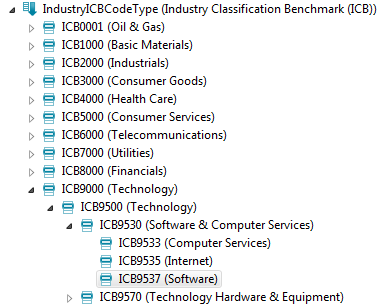
\includegraphics[width=9cm]{hierarchicalcodetype.png}
\caption{A hierarchical code type class shown in the Scout SDK.}
\figlabel{hierarchicalcodetype}
\end{figure}

The corresponding code for the ICB code type is provided in \lstref{codetype.hierarchical} where its hierarchical nature is reflected by method \java{getConfiguredIsHierarchy}. 
The actual hierarchical codes are then implemented as nested inner code classes that are derived from Scout class \java{AbstractCode}. 
See \figref{hierarchicalcodetype} for a screenshot of the partially expanded ICB code type class in the Scout SDK. 

% ........................................................................... %
\subsection{Loading Codes Dynamically}

Although codes types remain mostly static in their nature, they do evolve over time in any real world application. 
Requiring that all codes are statically defined in the application's code base would result in the necessity to update the code base for every change of a code required by the business. 
Clearly, such a setup is not sustainable and this is why Scout allows to dynamically update the set of codes contained in a code type.

\lstinputlisting[
  label=\lstlabel{codetype.addcodes},
  caption=Adding codes dynamically in method \java{execLoadCodes}.,
  index={execLoadCodes,Code Type|Load Codes Dynamically},
  linerange={21-51,195-211},
  float
]
{../code/widgets/org.eclipse.scout.widget.shared/src/org/eclipse/scout/widget/shared/services/code/ColorsCodeType.java}

At startup of a Scout application the codes of all defined code types are loaded into memory. 
For this, Scout internally calls method \java{loadCodes} for each code type class derived from class \java{AbstractCodeType}. 
In this method Scout first creates objects representing the statically defined codes and then dynamically adds additional codes in method \java{execLoadCodes}. 
By overriding this method, a code type class can dynamically add codes from any external sources. 
An example for the dynamic loading of codes is provided in \lstref{codetype.addcodes}. 
Please note that this code snipped only illustrates the principle and does therefore not access any external web services or databases. 

As codes have IDs and can be defined both statically in code and dynamically from external data, conflicting definitions of codes are inevitable. 
In the Scout framework these conflicts are resolved in method \java{execOverrideCode}. 
In the default implementation provided by class \java{AbstractCodeType}, priority is given to the dynamically defined code. 
Only attributes that are undefined for the dynamic code are copied from the static code definition. 
This logic can be changed for any code type by simply overriding method \java{execOverrideCode} with the desired behaviour. 
In the example provided in \lstref{codetype.addcodes} the code with ID \java{Color.YELLOW} is defined both statically and dynamically. 
As a result, the translated text for key \java{"YellowDynamic"} is shown in the user interface as it has priority over the statically defined text key \java{"Yellow"}. 

To have access to all codes at runtime, Scout provides the convenience accessor \java{CODES}. 
This accessor encapsulates the access to the \java{ICodeService} and provides a number of useful methods. 
% TODO where are the code services? widget has localcodeservice in client, registered in plugin.xml of client
% TODO helloworld does not seem to have registered a code service in shared or server or client. why not???
At startup, all codes are loaded and cached in the applications client session using method \java{getAllCodeTypes}. 
And for a class \java{MyCodeType}, all its codes can be retrieved by \java{CODES.getCodeType(MyCodeType.class).getCodes()}. 

% --------------------------------------------------------------------------- %
\section{Lookup Calls and Services}

Lookup calls are are used to look up lists of lookup rows in the form of key-text pairs. 
The list of lookup rows returned is usually defined by some search criteria. 
When the look up is triggered by a key, only a single element is returned. 
And when a string is provided as a search criteria, the returned list typically contains the lookup rows that contain the given search text as a substring. 

For lookup calls two main use cases exist. 
In the first case, the lookup data is locally available, not too large and can be kept in memory. 
In this situation, the lookup data can be directly created in the call itself. 
As an example, you may consider a lookup call where the lookup data is based on a code type.
In the other case, the lookup data is dynamic in nature, the amount of data is large and needs to be read from some external source, such as a database or a web service. 
To access large amounts of external data, a lookup call typically invokes a so called lookup service that is providing the necessary data. 
This is exactly the scenario that was used in the ''My Contacts�� application of the book's first part in \secref{adding_the_smartfield}. 
In the contact form of that application, a company smart field is used to let the user select a specific entry from a list of companies. 
And in turn, this smart field uses a company lookup call that is backed by a company lookup service. 
This lookup service then accesses a database to create the list of companies required for the company smart field. 

in the text below
(0) general aspects: 
    * getDataBy{Key|Text|Rec?|All}
	* additional properties as constraints to the result set: master field
	* for a specific implementation additional properties can be added with getters/setters ? -> yes as they are passed to services as bind variables
(1) local lookup calls in the client plugin
(2) lookup calls in the shared plugin
(3) lookup services are only mentioned here for completeness. full discussion in book part 3 for scout server? or not? probably needs to be here ...

\lstinputlisting[
  label=\lstlabel{lookup.local.simple},
  caption=A simple local lookup call defining it's entries in method \java{execCreateLookupRows}.,
  index={execCreateLookupRows,Lookup Call|Local Lookup Call},
  linerange={17-30},
  float
]
{../code/widgets/org.eclipse.scout.widget.client/src/org/eclipse/scout/widget/client/services/lookup/FontStyleLookupCall.java}

\lstinputlisting[
  label=\lstlabel{lookup.local.simple},
  caption=A local code lookup call. This lookup removes inactive codes in the lookup data.,
  index={Code Lookup Call},
  linerange={14-36},
  float
]
{../code/widgets/org.eclipse.scout.widget.client/src/org/eclipse/scout/widget/client/services/lookup/EventTypeLookupCall.java}

TODO: fix \figref{lookup_call}: MyLookupService extends AbstractLookupService and implements IMyLookupService that extends ILookupService which 

\begin{figure}
\includediagram{10cm}{lookup_call}
\caption{Implementing a lookup call with a corresponding lookup service. Scout framework components are shown in orange, user code in blue.}
\figlabel{lookup_call}
\end{figure}

 
\noindent Existing Documentation
\begin{itemize}
  \item presentation: \url{http://wiki.eclipse.org/images/c/c9/20111102_EclipseConEurope2011-EclipseScout-DiscoverThePotential.pdf}
  \item tutorial: \url{https://wiki.eclipse.org/Scout/Tutorial/Lookup_Calls}
  \item tutorial minicrm: \url{https://wiki.eclipse.org/Scout/Tutorial/4.0/Minicrm/Lookup_Calls_and_Lookup_Services}
  \item concept wiki: \url{http://wiki.eclipse.org/Scout/Concepts/LookupCall}
  \item concept wiki: \url{http://wiki.eclipse.org/Scout/Concepts/Lookup_Service}
  \item forum: \url{http://www.eclipse.org/forums/index.php/t/279108/}
  \item javadoc lookupcall: \url{https://eclipse.googlesource.com/scout/org.eclipse.scout.rt/+/Luna_RC3/org.eclipse.scout.rt.shared/src/org/eclipse/scout/rt/shared/services/lookup/LookupCall.java}
  \item javadoc lookuprow: \url{https://eclipse.googlesource.com/scout/org.eclipse.scout.rt/+/Luna_RC3/org.eclipse.scout.rt.shared/src/org/eclipse/scout/rt/shared/services/lookup/LookupRow.java}
  \item javadoc codelookupcall \url{https://eclipse.googlesource.com/scout/org.eclipse.scout.rt/+/Luna_RC3/org.eclipse.scout.rt.shared/src/org/eclipse/scout/rt/shared/services/lookup/CodeLookupCall.java}
  \item javadoc locallookupcall \url{https://eclipse.googlesource.com/scout/org.eclipse.scout.rt/+/Luna_RC3/org.eclipse.scout.rt.shared/src/org/eclipse/scout/rt/shared/services/lookup/LocalLookupCall.java}
  \item javadoc ilookupservice \url{https://eclipse.googlesource.com/scout/org.eclipse.scout.rt/+/Luna_RC3/org.eclipse.scout.rt.shared/src/org/eclipse/scout/rt/shared/services/lookup/ILookupService.java}	
  \item javadoc lookupservices \url{https://eclipse.googlesource.com/scout/org.eclipse.scout.rt/+/Luna_RC3/org.eclipse.scout.rt.server/src/org/eclipse/scout/rt/server/services/lookup/}
\end{itemize}

  * lookup service
  * sqllookup service


% --------------------------------------------------------------------------- %
\section{Permissions}

needs text, topic is relevant for client, server, and security. what to present where to be decided

\noindent Existing Documentation
\begin{itemize}
  \item how-to wiki: \url{http://wiki.eclipse.org/Scout/HowTo/3.8/Create_Permissions}
  \item concept wiki: \url{http://wiki.eclipse.org/Scout/Concepts/Permission}
  \item forum: \url{http://www.eclipse.org/forums/index.php/t/243966/}
\end{itemize}

% --------------------------------------------------------------------------- %
\section{Form Data Objects}
needs text, explain that form data objects are data transfer objects

\noindent Existing Documentation
\begin{itemize}
  \item form data/dto \url{http://www.eclipse.org/forums/index.php/t/169334/}
\end{itemize}

\subsection{Data Binding}
needs text, this is about Form Data Export and Import

\subsection{Automatic Updates by the Scout SDK}
needs text

\subsection{Manual Form Data Updates}
needs text

% =========================================================================== %
\chapter{Client components}
needs text

% --------------------------------------------------------------------------- %
\section{Client Model}

needs text
\begin{figure}[!htb]
\centering
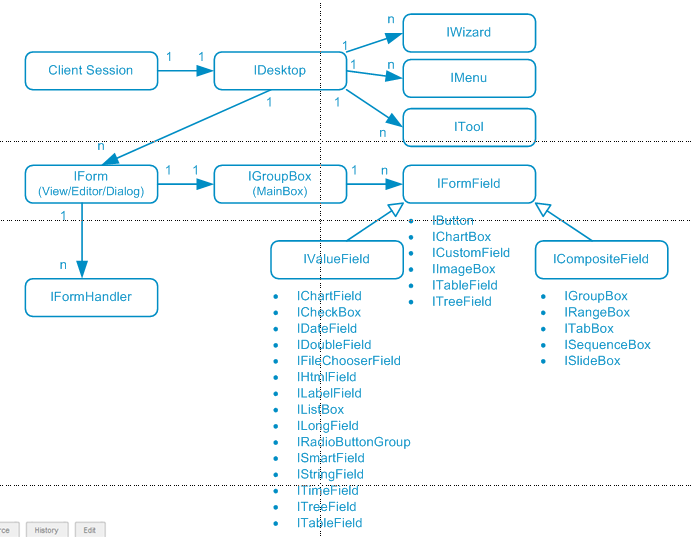
\includegraphics[width=0.8\textwidth]{scoutclientmodel.png}
\caption{A class diagram for the Scout's client model.}
\label{fig:scoutclientmodel}
\end{figure}

% --------------------------------------------------------------------------- %
\section{Splash Screen}
needs text

% --------------------------------------------------------------------------- %
\section{Login Box}
needs text

% --------------------------------------------------------------------------- %
\section{Client Session}
needs text

% --------------------------------------------------------------------------- %
\section{Desktop}
needs text

\noindent Existing Documentation
\begin{itemize}
  \item concept wiki \url{http://wiki.eclipse.org/Scout/Concepts/Desktop}
\end{itemize}

\subsection{Info Dialog}
needs text

\subsection{Toolbar}
needs text

\noindent Existing Documentation
\begin{itemize}
  \item forum: feature request \url{http://www.eclipse.org/forums/index.php/t/366440/}
  \item concept wiki \url{http://wiki.eclipse.org/Scout/Concepts/Tool}
\end{itemize}

\subsection{Status Line}
needs text

% --------------------------------------------------------------------------- %
\section{Menus}
needs text

\noindent Existing Documentation
\begin{itemize}
  \item concept wiki \url{http://wiki.eclipse.org/Scout/Concepts/Menu}
  \item forum: hard coded swt menues \url{http://www.eclipse.org/forums/index.php/t/236071/}. is this still an issue with scout kepler?
\end{itemize}

% --------------------------------------------------------------------------- %
\section{Outlines}
needs text

\noindent Existing Documentation
\begin{itemize}
  \item concept wiki \url{http://wiki.eclipse.org/Scout/Concepts/Outline}
\end{itemize}

% --------------------------------------------------------------------------- %
\section{Tools}
needs text

	
% --------------------------------------------------------------------------- %
\section{Forms}
needs text

\noindent Existing Documentation
\begin{itemize}
  \item concept wiki \url{http://wiki.eclipse.org/Scout/Concepts/Form}
  \item concept wiki form handler\url{http://wiki.eclipse.org/Scout/Concepts/Form_Handler}
  \item how-to wiki \url{http://wiki.eclipse.org/Scout/HowTo/3.8/Open_a_Form_in_a_View}
  \item forum: layout manager \url{http://www.eclipse.org/forums/index.php/t/404048/}
  \item forum: life cycle \url{http://www.eclipse.org/forums/index.php/t/369890/}
\end{itemize}

	* form validation

% --------------------------------------------------------------------------- %
\section{Form Fields}
needs text

Every Scout form contains one or several form fields.
Form fields therefor represent the basic building blocks of a forms content. 
Depending on their nature, form fields can display information, accept user input or act as container holding inner form fields.
As such container fields can hold inner container fields it is possible to create forms that meet compolex requirements.

\noindent Existing Documentation
\begin{itemize}
  \item concept wiki (links) \url{http://wiki.eclipse.org/Scout/Concepts/Client_Plug-In#Form_fields}
  \item concept wiki screenshots \url{http://wiki.eclipse.org/Scout/Concepts/Field}
\end{itemize}

% --------------------------------------------------------------------------- %
\subsection{Common Aspects}
needs text

\noindent Existing Documentation
\begin{itemize}
  \item forum: label position \url{http://www.eclipse.org/forums/index.php/t/369109/}
\end{itemize}

* model component
* ui component
* extension point registration

* model
* label
* value
* exec methods
* field validation

% --------------------------------------------------------------------------- %
\section{Trees}
needs text

    * tree nodes
	* tree form
	* tree field

	
% --------------------------------------------------------------------------- %
\section{Pages}
needs text

\noindent Existing Documentation
\begin{itemize}
  \item how-to wiki: \url{http://wiki.eclipse.org/Scout/HowTo/3.8/Display_images_in_a_table_page}	
  \item concept wiki: \url{http://wiki.eclipse.org/Scout/Concepts/Page}
  \item forum: pages linking to forms \url{http://www.eclipse.org/forums/index.php/t/367595/}
  \item forum: changing page icons \url{http://www.eclipse.org/forums/index.php/t/262151/}
\end{itemize}

    * page with table
	* page with nodes

	
% --------------------------------------------------------------------------- %
\section{Search Forms}
needs text

\noindent Existing Documentation
\begin{itemize}
  \item forum: position of search form \url{http://www.eclipse.org/forums/index.php/t/353895/}
  \item forum: statement builder stuff \url{http://www.eclipse.org/forums/index.php/t/165805/}
\end{itemize}

% --------------------------------------------------------------------------- %
\section{Tables}
needs text

\noindent Existing Documentation
\begin{itemize}
  \item forum: editable column \url{http://www.eclipse.org/forums/index.php/t/220019/}
  \item forum: default visibility of columns \url{http://www.eclipse.org/forums/index.php/t/166052/}
  \item forum: row deletion \url{http://www.eclipse.org/forums/index.php/t/210744/}
\end{itemize}

	* context menues
	* editable tables
    * column types

\subsection{Image Columns}
needs text

\noindent Existing Documentation
\begin{itemize}
  \item forum: \url{http://www.eclipse.org/forums/index.php/t/369626/}
\end{itemize}

\subsection{HTML inside Table Cells}
needs text

\noindent Existing Documentation
\begin{itemize}
  \item forum: \url{http://www.eclipse.org/forums/index.php/t/370714/}
  \item forum: summary row \url{http://www.eclipse.org/forums/index.php/t/235749/}
\end{itemize}

\subsection{Table Status Bar}
nees text

\noindent Existing Documentation
\begin{itemize}
  \item forum: \url{http://www.eclipse.org/forums/index.php/t/367326/}
\end{itemize}

\subsection{Injecting Columns at Runtime}
needs text

\noindent Existing Documentation
\begin{itemize}
  \item forum: \url{http://www.eclipse.org/forums/index.php/t/364715/}
  \item forum : dynamic columns \url{http://www.eclipse.org/forums/index.php/t/216731/}
\end{itemize}

% --------------------------------------------------------------------------- %
\section{Workflows and Wizards}
Needs text

\noindent Existing Documentation
\begin{itemize}
  \item concept wiki \url{http://wiki.eclipse.org/Scout/Concepts/Wizard}
  \item forum: \url{http://www.eclipse.org/forums/index.php/t/391607/}
  \item forum: \url{http://www.eclipse.org/forums/index.php/t/382579/}
  \item forum: \url{http://www.eclipse.org/forums/index.php/t/366971/}
\end{itemize}

% =========================================================================== %
\chapter{The Widgets Demo Application}
\chalabel{widgetsdemo}

This chapter introduces the "Scout Widgets Demo App".
The purpose of this demo application is to present Scout's most commonly used UI widgets. 
Therefore, the application does not contain any business logic but only serves as a hands-on reference on how to use and configure Scout UI widgets.

It is interesting to note that the widget demo application works out-of-the-box with any of the currently supported UI technologies. 
This means that with the same code base the widget demo application is capable to run as a native desktop application, as a web application in browsers, as well as on touch-enabled mobile devices. 
Comparing individual aspects of the the desktop application with its mobile/tablet version reveals the default strategies used to map desktop widgets to the substantially different usage/form factor found on mobile devices. 
Please observe that for the complete widget application only a handful of lines of code actually depend on a specific UI technology. 
The interested reader can easily verify this by searching the application's code for the occurrences of class \java{UserAgentUtility}.

In the text below the organisation of the widget demo application is first described in \secref{widgetdemo_ui}. 
And in \secref{widgetdemo_architecture}, the setup in the form of a Scout client only application is explained.

% --------------------------------------------------------------------------- %
\section{The User Interface}
\seclabel{widgetdemo_ui}

The application is organized into separate outlines for thematic groups of widgets. 
Each of the application's outline then presents a list of widgets in a navigation tree.
This is shown in \figref{widgetapp_github} for the \outline{Simple Widgets} that contains examples for simple UI widgets such as label fields or string fields.

\begin{figure}
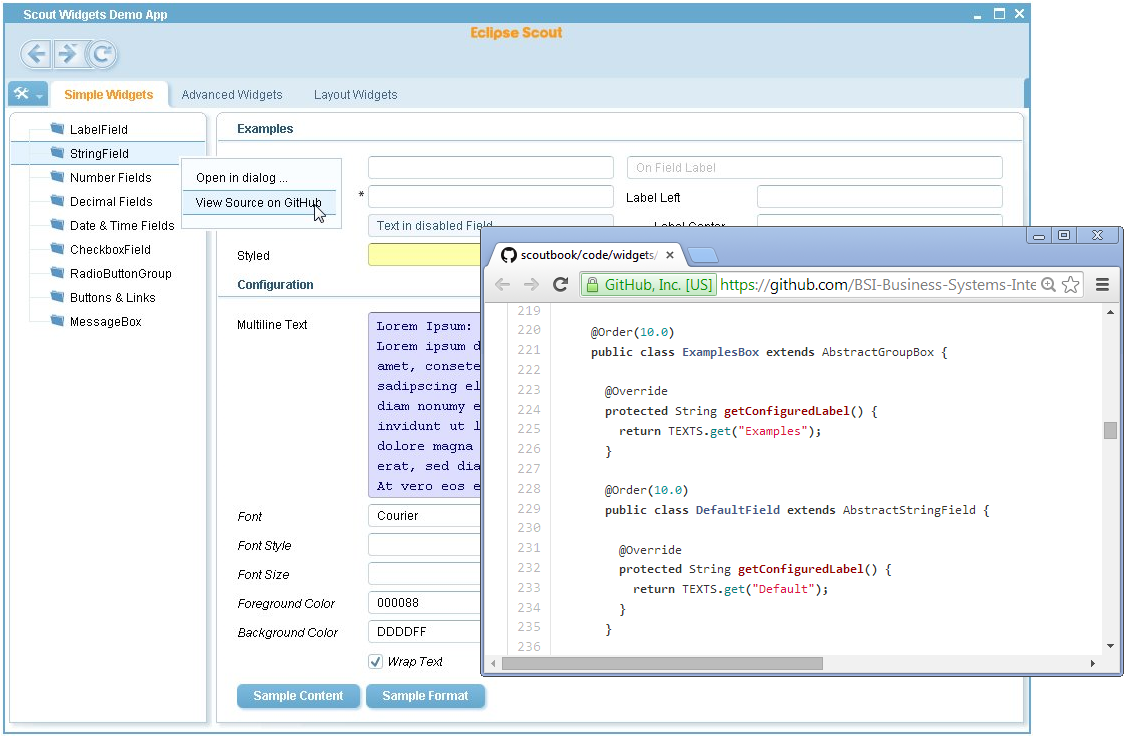
\includegraphics[width=14cm]{widgetapp_github_menu.png}
\caption{The "Scout Widgets Demo App". 
The widgets demo application features examples of the most commonly used Scout widgets.
For each widget shown, example use cases are presented in a individual form. 
As shown in the screenshot, the corresponding Scout source code is made available via the \contextmenu{View Source on GitHub}. }
\figlabel{widgetapp_github}
\end{figure}

For each UI widget a corresponding example form presents a number of typical use cases and configuration options. 
The example forms are designed to be independent from each other. 
It should therefore be possible to read and understand the source code of each example form with minimal effort.
Via the \contextmenu{Open in Dialog \dots} the content of the view is displayed in a modal scout form. 
As shown in \figref{widgetapp_github}, the complete source code for the selected form can be accessd via the \contextmenu{View Source on GitHub}.

\begin{figure}
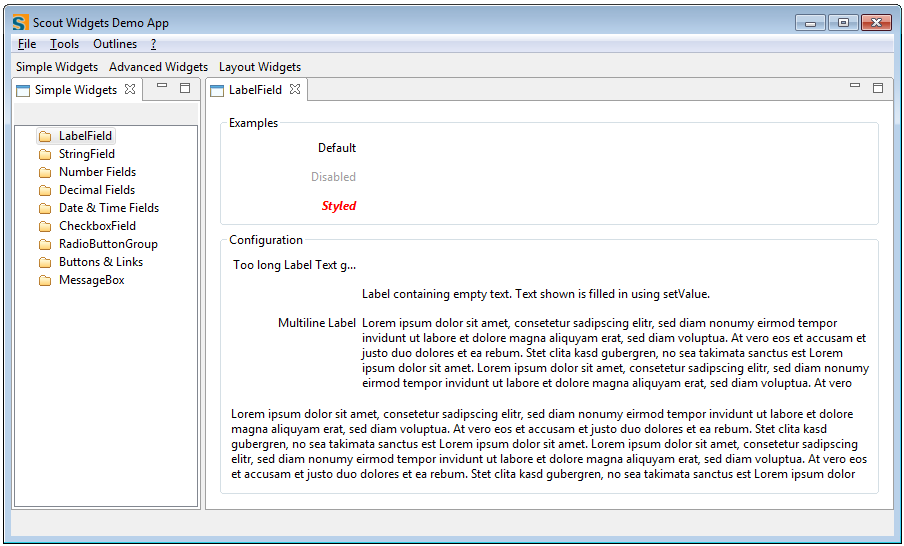
\includegraphics[width=14cm]{widgetapp_swt.png}
\caption{The "Scout Widgets Demo App" running as an SWT desktop application.}
\figlabel{widgetapp_swt}
\end{figure}

\begin{figure}
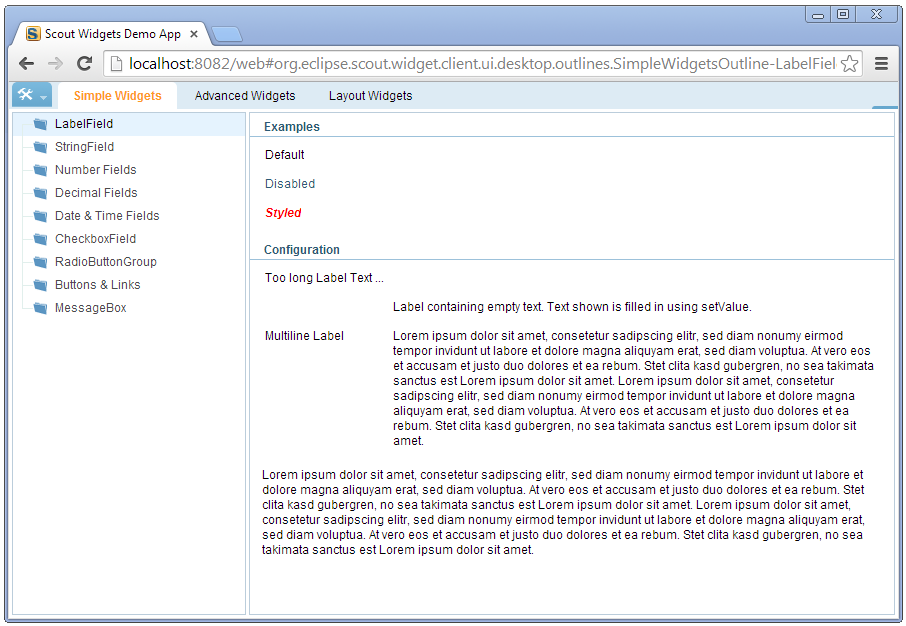
\includegraphics[width=14cm]{widgetapp_web.png}
\caption{The "Scout Widgets Demo App" running in the browser.}
\figlabel{widgetapp_web}
\end{figure}

The widget demo application can also be run as a native SWT desktop application. 
This is shown in \figref{widgetapp_swt}.
And the exact same application also runs in a browser as a web application shown in \figref{widgetapp_web}.

\begin{figure}
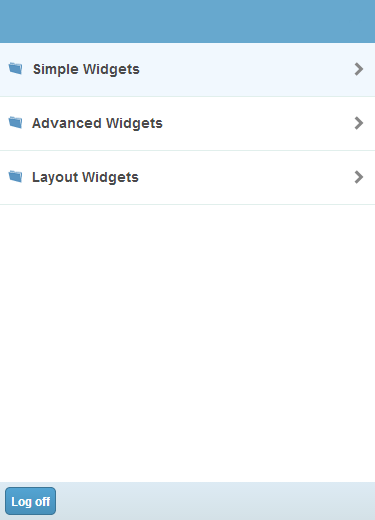
\includegraphics[width=4.5cm]{widgetapp_mobile1.png}
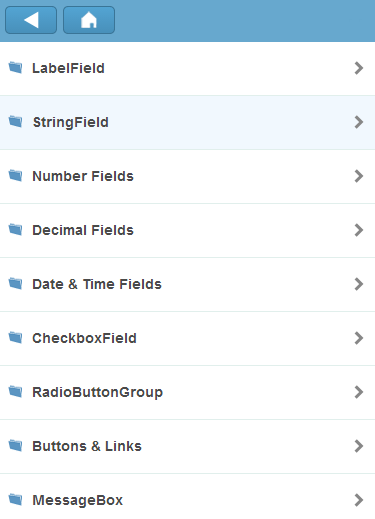
\includegraphics[width=4.5cm]{widgetapp_mobile2.png}
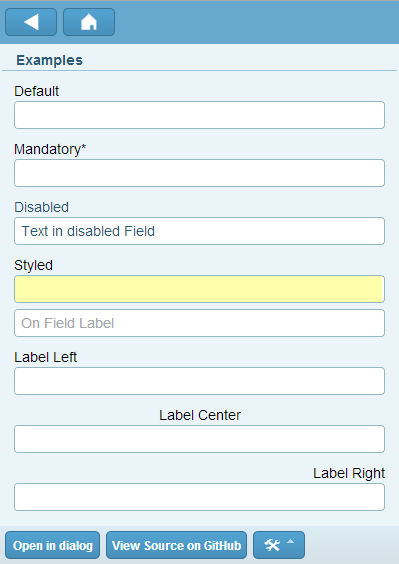
\includegraphics[width=4.5cm]{widgetapp_mobile3.png}
\caption{The "Scout Widgets Demo App" running on a mobile device. 
On the left, all outlines of the application are displayed on the home screen.
The screens shown in the middle allows to navigate through ''Simple Widgets'' outline while the selected ''StringField'' form is shown on the right.
}
\figlabel{widgetapp_mobile}
\end{figure}

In \figref{widgetapp_mobile}, the content of the widget demo application is shown on a mobile device. 
On the home screen of the mobile application, the available outlines are presented. 
When the user selects a specific outline, the associated navigation tree is then shown as a scrollable list. 
Finally, when the user selects a specific widget, the associated example form is shown. 

% --------------------------------------------------------------------------- %
\section{Client Only Architecture}
\seclabel{widgetdemo_architecture}

As the sole purpose of the widget demo application is to demonstrate the usage of the UI elements provided by the Scout framework, no server side data access and/or business logic is required. 
Therefore, the widget demo application has been designed as a client only application. 
As a side effect, the architecture of this widget application may also be used as a template to build similar client only applications with the Scout framework. 
It is important to note that this architecture can only be recommended for very simple applications. 
For more complex software packages, for example personal digital archives or private accounting software, it is not recommended to implement the business logic and the access to the database in the application's client plugin. 
A much cleaner approach is to take advantage of the offline support provided by the Scout framework. 
As in typical Scout client server projects, the presentation logic can be implemented in the client plugin and business logic and access to a (local) database are located in the server plugin. 
A detailed description of this setup including step-by-step instructions is available on the Scout Wiki\footnote{
Standalone Client with DB Access: \url{http://wiki.eclipse.org/Scout/HowTo/Create_a_Standalone_Client_with_DB_Access}
}.
In the text below the client only setup of the widget demo application is explained by looking at the main differences to the setup of the ``Hello World'' application introduced in \charef{helloworld}. 

\lstinputlisting[
  label=\lstlabel{demoapp.clientsession},
  caption=The setup of the client session in the Scout widget demo application.,
  index={ClientSession,execLoadSession},
  linerange={25-33},
  float
]
{../code/widgets/org.eclipse.scout.widget.client/src/org/eclipse/scout/widget/client/ClientSession.java}

The most obvious difference of the widget demo application to the ``Hello World'' client server example is the missing server (plugin). 
Consequently, the widget demo application also does not need a service tunnel to handle client server communication.
As the setup of this service tunnel is typically initiated in method \java{execLoadSession} of the client's \java{ClientSession} class, 
the setup of the service tunnel has been commented out in the widget demo application according to \lstref{demoapp.clientsession}. 

The next difference between typical Scout applications and the widget demo lies in the handling of code types and codes. 
Accessing code types and codes is the responsibility of the server's \java{CodeService} class in Scout applications. 
As the widget demo does not have a server but we still want to work with codes and code types, a \java{LocalCodeService} class has been added to the client's plugin. 

The last difference of note between the ``Hello World'' example and the widget demo application lies in the implementation of the form handler classes. 
In the desktop form's view handler of the ``Hello World'' application the data to be displayed is retrieved via the server's \java{DesktopService} as shown in \lstref{helloworld.viewhandler}. 
As the forms of the widget demo application do not load/persist any data from/to a server, no such logic is required in the form handlers and the corresponding classes remain empty. 

% =========================================================================== %
\chapter{Simple Widgets}
\chalabel{simplewidgets}

This chapter presents the most commonly used Scout widgets based on the widget demo application introduced above. 
For each widget the most frequently observed use cases are presented and illustrated with the widget specific example forms. 
And exemplary code snippets taken from the widget application help to close the loop to the actual implementation of these widgets in the applications source code.

% --------------------------------------------------------------------------- %
\section{Label Fields}

Label fields are used to place a read only text anywhere in a Scout form. 
As shown in the configuration section of \figref{labelfield} such texts can occupy the typical area assigned to a label field on the left, the area typically assigned to data entry on the right or on both sides.
The form shown in \figref{labelfield} is implemented in class \java{LabelFieldForm} of the Scout widget application.

\begin{figure}
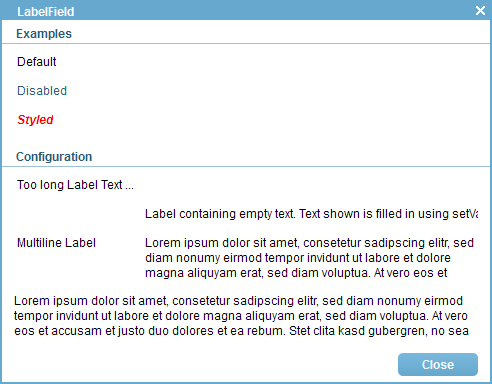
\includegraphics[width=10cm]{labelfield.png}
\caption{Scout fields and example use cases. 
In the examples section of the form the standard usage of label fields is shown.
To display text over the whole width of a column or in the area right to the label use method \java{setValue} as shown in the configuration section of the form.}
\figlabel{labelfield}
\end{figure}

To set the label text in the default area method \java{getConfiguredLabel} is used. 
If the label text is too long for the reserved area the label gets truncated with trailing \dots.
The complete label text is then shown in a tooltip.

As for any form field derived from \java{AbstractFormField}, a number of \java{getConfigured*} styling properties exist for label fields.
Most of these styling properties can directly be set in the Scout Object Properties view.
A subset of these properties are shown in the list below.

\begin{itemize}
  \item Label Position
  \item Label Horizontal Alignment
  \item Label Foreground Color
  \item Label Background Color
  \item Label Font
\end{itemize}

\lstinputlisting[
  label=\lstlabel{field.label.value},
  caption=A simple LabelField.,
  index={AbstractLabelField,Label Field},
  linerange={66-73},
  float
]
{../code/widgets/org.eclipse.scout.widget.client/src/org/eclipse/scout/widget/client/ui/forms/LabelFieldForm.java}

To display text in the right hand area an empty string can be used as label text and the text for the value area of the label field can be set with method \java{setValue} in method \java{execInitField} according to \lstref{field.label.value}.

\lstinputlisting[
  label=\lstlabel{field.label.multiline},
  caption=A label field displaying multi-line text that covers the whole width of a column.,
  index={AbstractLabelField,Label Field},
  linerange={168-195},
  float
]
{../code/widgets/org.eclipse.scout.widget.client/src/org/eclipse/scout/widget/client/ui/forms/LabelFieldForm.java}

To display multiline text across both the label and the value area a combination of label field properties has to be used.
See \lstref{field.label.multiline} for the configuration used in the last label field shown in \figref{labelfield}.

% --------------------------------------------------------------------------- %
\section{String Fields}

String fields are used to enter simple text strings. 
In addition, string fields are also useful to enter multiline text or capture masked input.
The form shown in \figref{stringfield} is implemented in class \java{StringFieldForm} of the Scout widget application.

\begin{figure}
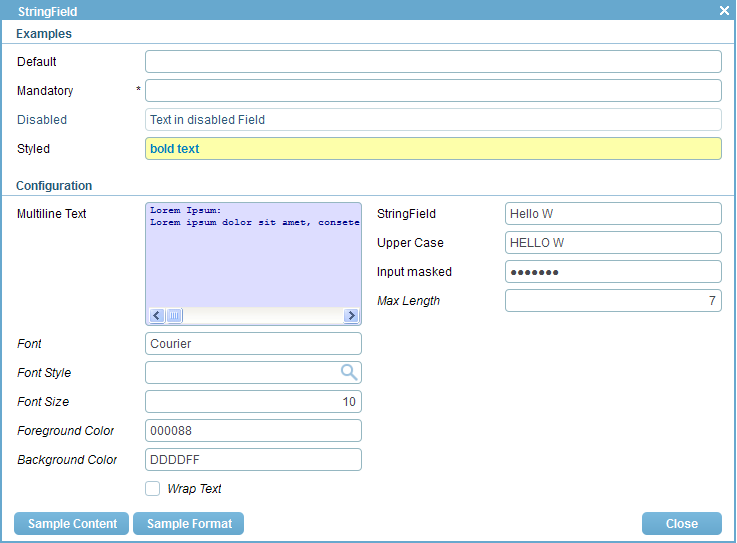
\includegraphics[width=15cm]{stringfield.png}
\caption{String fields and example use cases.
Text content shown in disabled fields can be read and copied to the clipboard, but not edited.
In multi line string fields the text can be displayed as entered or the text may be wrapped to fit into the available column with.}
\figlabel{stringfield}
\end{figure}

Some of the most typical use cases for string fields are represented in the examples section of \figref{stringfield}.
In the configuration section of the form a multiline text field is shown.
As in the case of the label text, font and color styling possibilities are available for the text shown in a string field. 
Clicking on the \button{Sample Format} and on the \button{Sample Content} prefills some of the fields to create the effect shown in \figref{stringfield}.

In the case of multi line string fields, the field can be configured to either display text lines as they have been entered or wrapped to fit into the available width of the field. 
This property can be set with the string field's method \java{getConfiguredWrapText} or dynamically with method \java{setWrapText}. 
Please note that changing this property dynamically at runtime currently only works with the SWT and the Swing rendering components.

\lstinputlisting[
  label=\lstlabel{field.string.masked},
  caption=A masked string field.,
  index={AbstractStringField,String Field},
  linerange={595-607},
  float
]
{../code/widgets/org.eclipse.scout.widget.client/src/org/eclipse/scout/widget/client/ui/forms/StringFieldForm.java}

Additional use cases for the string field are shown in the right column of the configuration section of the string field demo form. 
Specific string fields are located for the default case, a string field only accepting upper case letters, and a masked field. 
To code to represent the masked string field is provided in \lstref{field.string.masked}.
Independent of what the user is typing the masked field keeps the entered content visually hidden. 
In contrast to all other forms of string fields, the content cannot be copied to the system clipboard.
It can only be accessed programmatically with the \java{getValue} method of the string field.

String fields also allow for the configuration of the maximum length of the text that can be entered into the field. 
In its default configuration, a maximum number of 4'000 characters can be entered into a string field. 
Using method \java{setMaxLength} this limit can be updated dynamically at runtime. 
Alternatively, this limit can also be set in method \java{getConfiguredMaxLength}. 

% --------------------------------------------------------------------------- %
\section{Number Fields}

For entering numbers, Scout provides three different fields.
Depending on the valid range of numbers that may be entered, an integer field, a long field or a big integer field best matches the given use case.
These fields are represented by the classes \java{AbstractIntegerField}, \java{AbstractLongField} and \java{AbstractBigIntegerField}, each one of them extinding class \java{AbstractNumberField}.

\begin{figure}
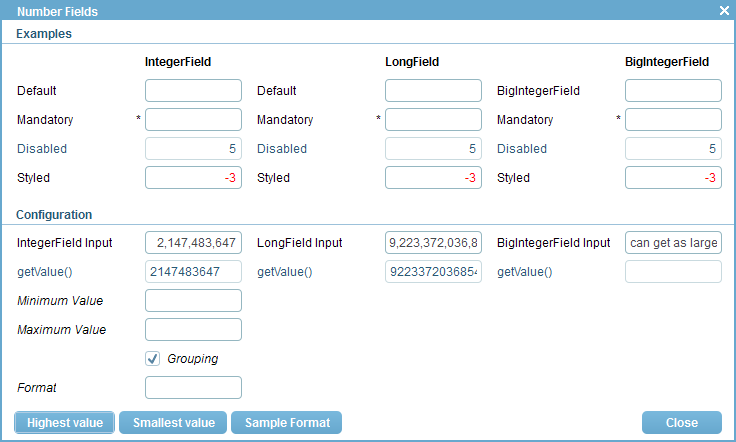
\includegraphics[width=15cm]{numberfield.png}
\caption{Number fields and example use cases.
Distinct number fields are available for \java{Integer}, a \java{Long} or a \java{BigInteger} value classes.
}
\figlabel{numberfield}
\end{figure}

The form \java{NumberFieldsForm} of the Scout widget application shown in \figref{numberfield} contains examples for all three number field types.
Separate buttons are available to demonstrate the use of the minimum and the maximum value a number field can hold.
In the case of the \field{BigInteger}, arbitrarily large or small values may be entered. 
See \lstref{field.integer.input} for the code corresponding to the input integer field in the configuration section of the example form.

\lstinputlisting[
  label=\lstlabel{field.integer.input},
  caption=A simple Integer field.,
  index={AbstractIntegerField,Integer Field},
  linerange={510-517},
  float
]
{../code/widgets/org.eclipse.scout.widget.client/src/org/eclipse/scout/widget/client/ui/forms/NumberFieldsForm.java}

As already indicated by the class names of the three number fields, the fields serve to enter values that fit into the ranges defined by the Java classes \java{Integer}, \java{Long} and \java{BigInteger}.
To further restrict the bounds of valid numbers you may use the methods \java{getConfiguredMinValue} and \java{getConfiguredMaxValue}.
The effect of setting such bounds can be tested by entering values into the \field{Minimum Value} and the \field{Maximum Value} of the example form.
If, for example, a minimum value of 0 is entered in the \field{Minimum Value} and the user tries to enter the value -1 into one of the input fields, an error marker becomes visible on the input field. 
A tooltip with the text ''The value is too small; must be between 0 \dots'' further explains the issue to the user.
In such a case the value entered into the user interface is not propagated to the number field's value.
This is why the read only \field{getValue()} is not updated in such a case.

To textually format the entered numbers the grouping number field property can be used. 
In the example form the \checkbox{Grouping} can be used to control this property.
Ticking/unticking this checkbox will affect the three number input fields in the configuration section of the example form.

More extensive options to specify the formatting of the numbers is provided by the method \java{setFormat} of class \java{AbstractNumberField}. 
Method \java{setFormat} is accepting an argument of the Java class \java{DecimalFormat}. 
To demonstrate an example for such a format click on \button{Sample Format} in the example form. 
For more information please consult the Javadoc for class \java{DecimalFormat}.

% --------------------------------------------------------------------------- %
\section{Decimal Fields}

Scout provides two different form fields for entering decimal values. 
Depending on the required precision and range of values to be entered a double field or a big decimal field can be used. 
The two field types are represented by Scout's classes \java{AbstractDoubleField} and \java{AbstractBigDecimalField} and can hold values of the Java types \java{Double} and \java{BigDecimal} respectively. 
Both the double and the big decimal field extend class \java{AbstractDecimalField} which in turn extends class \java{AbstractNumberField}.

\begin{figure}
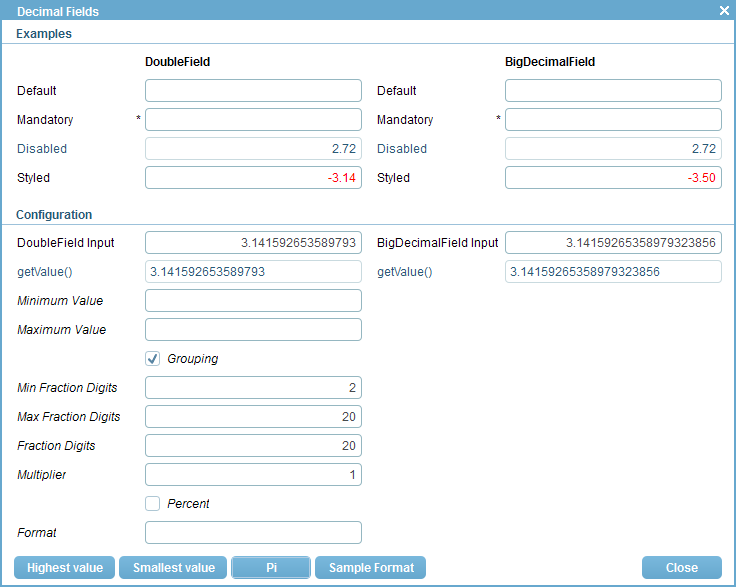
\includegraphics[width=15cm]{decimalfield.png}
\caption{Decimal fields and example use cases.
Distinct number fields are available for the \java{Double} and \java{BigDecimal} value classes.
}
\figlabel{decimalfield}
\end{figure}

The example form shown in \figref{decimalfield} demonstrates the usage and some of the available options to configure Scout's decimal fields.
This example form is defined in class \java{DecimalFieldsForm} of the Scout widget application. 

\lstinputlisting[
  label=\lstlabel{field.double.styled},
  caption=A styled decimal field holding Java \java{Double} values. Negative values are shown in red,
  index={AbstractDoubleField,Double Field},
  linerange={313-337},
  float
]
{../code/widgets/org.eclipse.scout.widget.client/src/org/eclipse/scout/widget/client/ui/forms/DecimalFieldsForm.java}

The styled double field in the example section of the form displays negative values in red and postive values in the default black color. 
This behaviour is implemented in method \java{execChangedValue} according to \lstref{field.double.styled}. 
The sample value shown initially is provided in the \java{execInitField} method. 
Setting the red foreground color explicitely is needed in method \java{execInitField} as the \java{execChangedValue} is only triggered after the initial form is displayed on the screen. 

For displaying and storing the fraction digits of decimal values three different properties exist. 
Two of them, the \java{getConfiguredMinFractionDigits} and the \java{getConfiguredMinFractionDigits} affect the optical representation of the decimal value. 
To configure the amount of fraction digits that is effectively represented the property \java{getConfiguredFractionDigits} is used. 
The need for three different properties might not be immediately clear. 
To illustrate the concept, let us look at an example use case where a decimal field always has to display exactely 3 fraction digits. 
Should the user provide more fraction digits we would like to capture this additional information up to 5 fraction digits. 

To configure this behaviour the following settings for this decimal field may be used.

\begin{itemize}
  \item \textit{Min Fraction Digits}: 3
  \item \textit{Max Fraction Digits}: 3
  \item \textit{Fraction Digits}: 5
\end{itemize}

If the user enters the text ''3.141592653589793'' into this field and tabs to the next field, the field will then display the text ''4.142'' but actually hold the value 3.14159. 
And if the user just enters a ''3'', the field will display ''3.000'' and hold the value 3.0.

Decimal fields can also be configured to enter percentages in a convenient way. 
For this use case the \property{Multiplier} can be set to 100 and the \property{Multiplier} to \java{true}. 
If the user now enters ''5'' into such a decimal field, it will show the text ''5\%'' and hold the value 0.05.

As in the case of number fields more extensive options to specify the formatting of the numbers is provided by \java{setFormat} method of the decimal field. 
Method \java{setFormat} is accepting an argument of the Java class \java{DecimalFormat}. 
To demonstrate an example for such a format click on \button{Sample Format} in the example form. 
For more information please consult the Javadoc for class \java{DecimalFormat}.

% --------------------------------------------------------------------------- %
\section{Date and Time Fields}

To work with date and time values Scout offers three dinstinct form fields. 
The \java{AbstractDateField} allows the user to enter a date and the \java{AbstractTimeField} is used to enter a time. 
The third field \java{AbstractDateTimeField} combines date and time entry into a single form field. 
Both classes \java{AbstractTimeField} and \java{AbstractDateTimeField} are extending the \java{AbstractDateField} field.

\begin{figure}
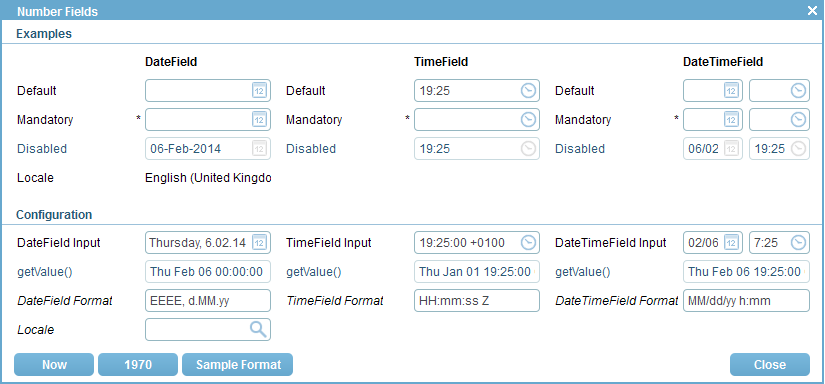
\includegraphics[width=15cm]{datetimefield.png}
\caption{Example use cases for a date, a time and a combined date/time field.
}
\figlabel{datetimefield}
\end{figure}

The form \java{DateTimeFieldsForm} of the Scout widget application shown in \figref{datetimefield} contains examples for the date and time fields of Scout.
Separate buttons are available to provide samle values and to demonstrate the formatting options for displaying date and time values.
Displaying dates and times is highly depending on the used locale.
That is why the currently used locale is shown in the example section of the form.

To enter date and time values the user can either click on the date and time icons/buttons provided by the fields or directly enter text into the fields. 
For entering dates the key arrows provide a number of shortcuts. 
Entering the currnt date can be done by pressing the \key{Up}. 
Once a day is entered in a date or a combined day time field, the \key{Up} and the \key{Down} can be used to step to the next/previous day. 
Simultaneously pressing the \key{Shift} or the \key{Ctrl} allows to step to the next/previous month or year.

\lstinputlisting[
  label=\lstlabel{field.datetime.disabled},
  caption=A disabled combined date time field initialized with the current time,
  index={AbstractDateTimeField,DateTime Field},
  linerange={448-465},
  float
]
{../code/widgets/org.eclipse.scout.widget.client/src/org/eclipse/scout/widget/client/ui/forms/DateTimeFieldsForm.java}

The code of the \java{DateTimeDisabledField} field shown in \lstref{field.datetime.disabled} represents the disabled combined date time in the example form. 
Before the form is opened Scout executes its \java{execInitField} method and sets the fields value to the current date and time. 

In the configuration section the local can be used at runtime to test the effect of the locale to displaying date and time fields. 
As changing the locale at runtime only works reliably in rich clients the field is only editable in the Swing or the SWT client. 
To specify the exact formatting of the displayed date and time values a specific format can be set in the \java{getConfiguredFormat} method of the date and time fields. 
Internally, Scout is using the provided string to create a Java \java{SimpleDateFormat} for formatting. 
Valid examples for the formatting are entered into the format fields of the example dialog by pressing the \button{Sample Formats}. 
The string ''EEEE'' shown in date field format field represents the day of the week as shown in configuration section of \figref{datetimefield}. 
As expected, the textual representation of the day of the week is depending on the used locale. 

% --------------------------------------------------------------------------- %
\section{Checkbox Fields}

Check boxes can be used to enter/represent simple boolean values. 
In Scout, check boxes are derived from class \java{AbstractCheckBox}. 

\begin{figure}
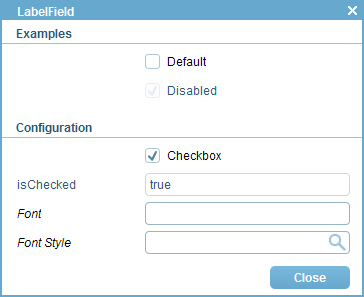
\includegraphics[width=7cm]{checkboxfield.png}
\caption{Check box field and example use cases.
}
\figlabel{checkboxfield}
\end{figure}

In the Scout widget application the use of check boxes is demonstrated in the form \java{CheckboxFieldForm} that is shown in \figref{checkboxfield}. 
To access the current value, Scout provides the method \java{isChecked} for check box fields. 
This naming reflects the boolean state of a check boxes and differs from the other Scout value fields that provide a \java{getValue} method.  

\lstinputlisting[
  label=\lstlabel{field.checkbox.disabled},
  caption=A disabled check box field initialized with a checked state,
  index={AbstractCheckBox,Check Box},
  linerange={144-163},
  float
]
{../code/widgets/org.eclipse.scout.widget.client/src/org/eclipse/scout/widget/client/ui/forms/CheckboxFieldForm.java}

A coding example is provided in \lstref{field.checkbox.disabled} for the disabled check box. 
The initial value is set in method \java{execInitField} using the method \java{setChecked}.

% --------------------------------------------------------------------------- %
\section{Radio Button Fields}

With radio buttons the user can select a single element out of a number of distinct choices. 
For this, a number of radio buttons may be placed into a radio button group field where a radio button group extends class \java{AbstractRadioButtonGroup}.
The contained individual buttons are extending class \java{AbstractRadioButton}.

\begin{figure}
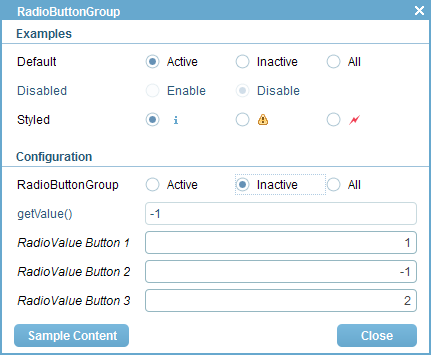
\includegraphics[width=9cm]{radiobuttonfield.png}
\caption{Radio buttons in a radio button group field and example use cases.
Assigning distinct values to the individual radio buttons allows to query the selected radio button.}
\figlabel{radiobuttonfield}
\end{figure}

\figref{radiobuttonfield} demonstrates the use of radio button groups in Scout. 
It is implemented in class \java{RadioButtonGroupFieldForm} of the Scout widget application. 
As shown in the example section of the form, radio buttons may have labes and/or icons assigned. 

\lstinputlisting[
  label=\lstlabel{field.radiobuttongroup},
  caption=A radio button group defined by a code type,
  index={AbstractRadioButtonGroup,Radio Button Group},
  linerange={186-202},
  float
]
{../code/widgets/org.eclipse.scout.widget.client/src/org/eclipse/scout/widget/client/ui/forms/RadioButtonGroupFieldForm.java}

The simplest way to define the content of a radio button group is by using its configuration properties \java{getConfiguredCodeType} or \java{getConfiguredLookupCall}. 
\lstref{field.radiobuttongroup} provides the implementation of ''Default�� radio button group \java{DefaultGroup}. 
This radio button group is typed by the generic parameter \java{Long} and the individual radio buttons are obtained from the code type \java{EventTypeCodeType} specified in method \java{getConfiguredCodeType}.
Please note that the \java{Long} type matches the key type of the codes in the \java{EventTypeCodeType}. 
The generic parameter used in the definition of a radio button group also determines the type that will be returned by the group's \java{getValue} method. 

\lstinputlisting[
  label=\lstlabel{field.radiobuttongroup.styled},
  caption=A complete radio button group with two radio buttons with individual radio values assigned,
  linerange={257-296},
  float
]
{../code/widgets/org.eclipse.scout.widget.client/src/org/eclipse/scout/widget/client/ui/forms/RadioButtonGroupFieldForm.java}

Alternatively, the individual buttons in a radio button group can also be defined as inner classes. 
This approach has been used for the ''Styled�� radio button group in the example section of the \java{RadioButtonGroupFieldForm}. 
The corresponding code is provided in \lstref{field.radiobuttongroup.styled}. 
The type of the value that is returned by the \java{getValue} method is defined on the radio button group. 
In the provided listing, the \java{StyledGroupBox} is configured to return a value of the type \java{Long}. 
Consequently, the individual radio buttons are returning radio values of the type \java{Long} as well in the \java{getConfiguredRadioValue} methods.
The field \java{PlaceholderField} in the radio button group only serves layouting purposes. 
Without this place holder field, the two radio buttons of the styled radio button group would be evenly distributed in the available space. 

% --------------------------------------------------------------------------- %
\section{Buttons and Links}

Buttons and links are used to trigger actions in Scout. 
Buttons come in two variations, normal push buttons and toggle buttons. 
While buttons have an associated label and/or icon, links can only have a label. 
Buttons extend class \java{AbstractButton} and links extend \java{AbstractLinkButton}. 

\begin{figure}
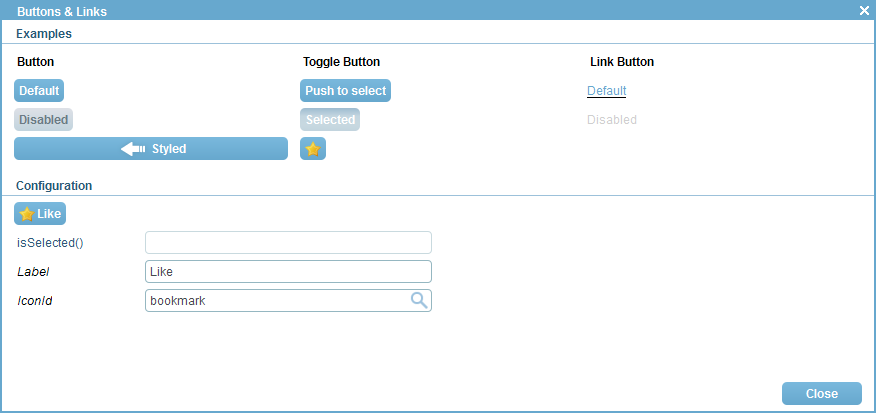
\includegraphics[width=15cm]{buttonlink.png}
\caption{Buttons and links may be placed on a Scout form to initiate actions.
Buttons may have an associated icon and/or a label.
Links only have a label.}
\figlabel{buttonlink}
\end{figure}

Example uses of buttons and links are shown in the form \java{ButtonLinkFieldsForm} of the Scout widget application shown in \figref{buttonlink}. 

\lstinputlisting[
  label=\lstlabel{field.button.styled},
  caption=A button with a label and an icon that horizontally stretches over the whole column,
  index={AbstractButton,Button},
  linerange={207-229},
  float
]
{../code/widgets/org.eclipse.scout.widget.client/src/org/eclipse/scout/widget/client/ui/forms/ButtonLinkFieldsForm.java}

In it's simplest form a button just extends class \java{AbstractButton} and overrides \java{getConfiguredLabel} to set the label. 
The example in \lstref{field.button.styled} also has an icon assigned and stretches over the whole column width. 
In addition, the example button overrides method \java{getConfiguredProcessButton} to return \java{false}. 
This has the effect that buttons (and links) appear at the exact location where they are defined in a field container. 
Otherwise, buttons (and links) are placed at the bottom of the container they are defined in. 

\lstinputlisting[
  label=\lstlabel{field.togglebutton},
  caption=A toggle button implementation that changes the label text depending on its toggled state,
  index={AbstractButton,Toggle Button},
  linerange={244-271},
  float
]
{../code/widgets/org.eclipse.scout.widget.client/src/org/eclipse/scout/widget/client/ui/forms/ButtonLinkFieldsForm.java}

The code of the default toggle button in the example form of the widget application is provided in \lstref{field.togglebutton}. 
To query the state of a toggle button method \java{isSelected} can be used. 

In the configuration section of the example form the use of mnemonics using the character \& is demonstrated. 
Please note, that this feature is not identically available across the different supported UI technologies. 
In the Swing UI shown in \figref{buttonlink} the label ''\&Toggle'' has the effect, that pressing the \altkey{T} key combination changes the toggle state of this button. 
In the case of the SWT UI the \key{alt} key is not necessary. 
Pressing the \key{T} changes the toggle state. 
In contrast to the Swing UI the letter 'T' is not underlined. 
To optically indicate shortcut letters in the SWT UI it is recommended to adapt the label from ''\&Toggle'' to ''[\&T]oggle''. 
The RAP UI does not currently support mnemonics on buttons. 

% --------------------------------------------------------------------------- %
\section{Message Boxes}

Message boxes are used to provide information to a user or ask the user simple yes/no questions. 
In Scout, class \java{MessageBox} provides a number of static convenience methods for this purpose. 
Additionally, message boxes are shown to the user in the case of a processing exception or a veto exception\footnote{
The processing exceptions type \java{ProcessingException} represents Scout's core exception class. 
The veto exception type \java{VetoException} is a direct subclass of the processing exception and is typically used in service calls for subjects with insuffiecient authorization. 
}. 

\begin{figure}
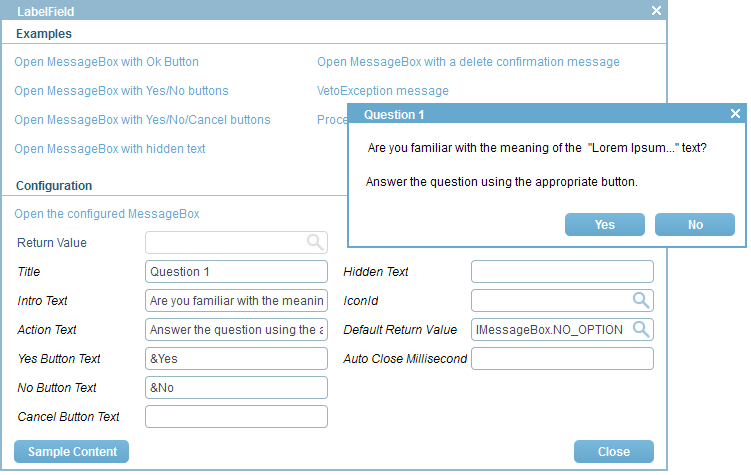
\includegraphics[width=14cm]{messagebox.png}
\caption{Message boxes are available for different use cases.
The message box shown in front is defined by the properties entered in the configuration section.}
\figlabel{messagebox}
\end{figure}

In the examples section of the \java{MessageBoxForm} form shown in \figref{messagebox} a number of links is provided. 
Clicking on any of these links opens a corresponding message box via the static convenience methods available with class \java{MessageBox}. 
For example, calling \java{MessageBox.showOkMessage(title, header, info)} opens a message box with a title, a header text and some additional information. 

\lstinputlisting[
  label=\lstlabel{field.openmessagebox},
  caption=Configuring and starting of a message box.,
  index={MessageBox,Configure a Message Box},
  linerange={434-453},
  float
]
{../code/widgets/org.eclipse.scout.widget.client/src/org/eclipse/scout/widget/client/ui/forms/MessageBoxForm.java}

In addition to the static convenience methods, message boxes can be configured to meet specific requirements by a number of parameters. 
These parameters are shown in \figref{messagebox} in the configuration section of the sample form \java{MessageBoxForm} of the Scout widget application.  
Clicking on the \button{Sample Content} will fill in example values for the message box parameters. 
The configured message box can them be started by clicking on the \link{Open the configured MessageBox}. 
This behaviour is implemented in the link's \java{execClickAction} method according to \lstref{field.openmessagebox}. 
The text below details the purpose of less evident message box properties.

Message box buttons only appear if an non-emtpy label text is assigned to the \property{Yes Button Text}, the \property{No Button Text} and \property{Cancel Button Text}. 
If the \property{hidden text} has a non-empty text assigned, an additional \button{Copy} will be added to the message box. 
An example use case is the case of elaborate error messages (or complete stack traces in cases where this does not negatively impact the application's security). 
Here the copy button allows to transport this text into the system clipboard. 
From the clipboard the user may decides to paste this text into an email to the companys help desk. 
The \property{default return value} specifies the return value of the message box if the box closes autmatically after the time provided in the \property{auto close millisecond} has passed. 
If the \property{auto close millisecond} is set to -1, the message box will not clause automatically. 

Once a message box is started with method \java{startMessageBox} the user interface is blocked until the user chooses any of the options or clicks the dialog away. 
The selected option is the provided by the method's return value. 
If the user closes the message box by hitting the \key{esc} or clicking on the icon to close a dialog, the start method of the message box will always return the value \java{CANCEL\_OPTION} of the \java{IMessageBox} interface.

% =========================================================================== %
\chapter{Advanced Widgets}
\chalabel{advancedwidgets}

This chapter presents some of the more complex widgets of the Scout framework. 
This set of widgets includes fields to handle and display list, tree and table data. 
Also included in this chapter are widgets to display images in both raster and vector formats.  
As in the previous chapter, for each described widget, screenshots of example use cases and corresponding code snippets are provided. 

% --------------------------------------------------------------------------- %
\section{List Box}

List boxes allow a user to select a subset of a predefined list of elements. 
The individual elements are displayed in the form of checkable options. 
To check or uncheck a specific element, the user may click on a element or press the \key{Space} when an element has the focus. 
To define the list of elements that are presented in a list box, code types or a lookup calls can be used. 
Example use cases using both code types and lookup calls for the definition of the presented elements are implemented in class \java{ListBoxForm} of the Scout widget application. 
See \figref{listbox} for a screenshot of the example form. 

\begin{figure}
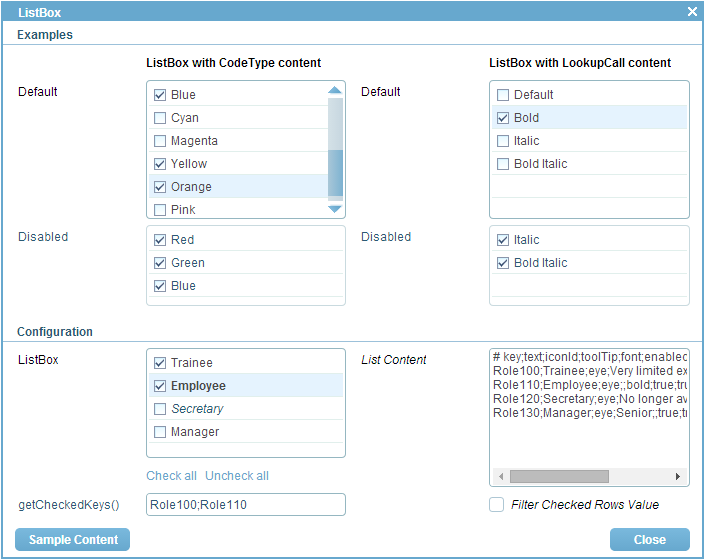
\includegraphics[width=14cm]{listbox.png}
\caption{List boxes to select elements represented by code types and lookup calls.}
\figlabel{listbox}
\end{figure}

\lstinputlisting[
  label=\lstlabel{field.listbox},
  caption=A simple ListBox field backed by a code type that returns elements of type \java{Color}.,
  index={ListBox},
  linerange={172-189},
  float
]
{../code/widgets/org.eclipse.scout.widget.client/src/org/eclipse/scout/widget/client/ui/forms/ListBoxForm.java}

In the example section of \figref{listbox} the list boxes in the left column retrieve the elements to be displayed from code types. 
And in the right column, the displayed elements are retrieved from lookup calls. 
The implementation of the top left \field{Default} is provided in \lstref{field.listbox}. 
List boxes are derived from class \java{AbstractListBox} and parameterized by the type of keys of the elements. 
Please note that the specified key type of a list box must match the key type of the elements provided by code types or lookup calls. 
In our example, the list box type \java{Color} matches the key type of the code type \java{ColorsCodeType} configured in method \java{getConfiguredCodeType}. 
	
In the \field{List Content} located on the right hand side of the configuration section of \figref{listbox} it is also possible to enter user defined content. 
After entering some example data and pressing the \key{Tab}, the user content is parsed and used to update the elements displayed in the \field{ListBox}. 
To get the initial example data shown in \figref{listbox}, use the \button{Sample Content} of the list box example form. 
Basically, the content of each text row is parsed into a lookup row according to the format provided in the first row of the sample content: \texttt{\# key;text;iconId;...}. 
The resulting lookup rows are then used to dynamically update the content of the lookup call associated with the \field{ListBox}. 
List boxes can be configured to only display the checked elements. 
For this, the configuration method \java{getConfiguredFilterCheckedNodes} may be used. 

\lstinputlisting[
  label=\lstlabel{field.getcheckedkeys},
  caption=Updating the \field{getCheckedKeys} whenever the use changes the selection of elements,
  index={ListBox.getCheckedKeys},
  linerange={356-379},
  float
]
{../code/widgets/org.eclipse.scout.widget.client/src/org/eclipse/scout/widget/client/ui/forms/ListBoxForm.java}

To access the currently selected elements of a list box method \java{getCheckedKeys} may be used. 
This is demonstrated in \lstref{field.getcheckedkeys} using the \field{getCheckedKeys} in the example form. 
In order to get notified for every change of the list box field, the list box field is registered as the master in method \java{getConfiguredMasterField}. 
The implementation of method \java{execChangedMasterValue} is then called whenever the state of the master field is changed. 
In the case of \lstref{field.getcheckedkeys}, the list of selected keys can be retrieved from the list box and shown in the \field{getCheckedKeys}. 

To read or write the content of a list box field from or to a form data on the server side, methods \java{getValue} and\java{setValue} have to be used. 
Both methods work with typed sets, requiring the type defined for the list box field.

% --------------------------------------------------------------------------- %
\section{Tree Box}

Tree box fields allow a user to select a subset of a predefined list of elements. 
The difference to list boxes lies in the organisation of the presented elements. 
Instead of presenting the elements as a list, a tree structure is used with tree box fields. 

To check and uncheck a specific element, the user may click on a element or press the \key{Space} when an element has the focus. 
In addition, tree boxes can also be configured to check or uncheck the complete sub tree when clicking on an element. 
To define the trees presented in tree boxes, hierarchical code types and lookup calls can be used. 
Example use cases for tree box fields are implemented in class \java{TreeBoxForm} of the Scout widget application.
A screenshot of the tree box example form is shown in \figref{treebox}. 

\begin{figure}
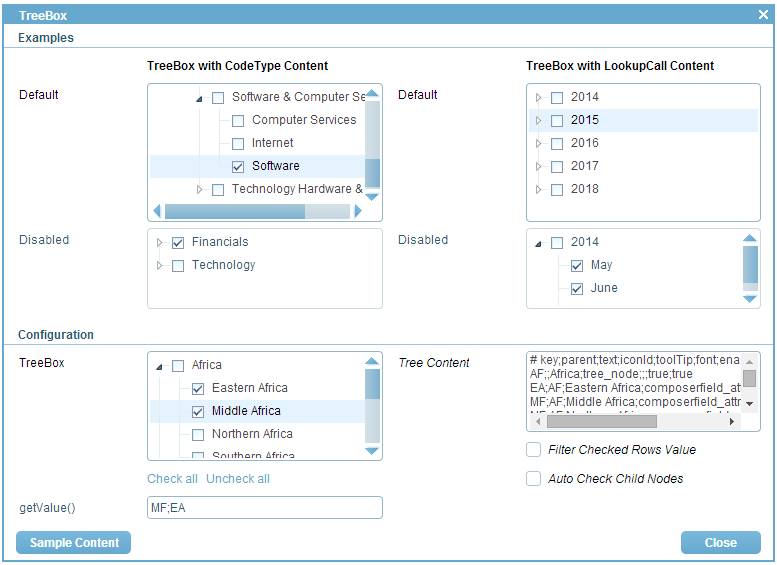
\includegraphics[width=14cm]{treebox.png}
\caption{Tree box fields displaying elements defined by hierarchical code types and lookup calls.}
\figlabel{treebox}
\end{figure}

\lstinputlisting[
  label=\lstlabel{field.treebox},
  caption=A simple TreeBox field backed by a lookup call that returns element keys of type \java{String}.,
  index={TreeBox},
  linerange={252-269},
  float
]
{../code/widgets/org.eclipse.scout.widget.client/src/org/eclipse/scout/widget/client/ui/forms/TreeBoxForm.java}

In the example section of \figref{treebox} the tree boxes in the left column retrieve the elements to be displayed from hierarchical code types. 
And in the right column, the displayed elements are retrieved from hierarchical lookup calls. 
The implementation of the top right \field{Default} is provided in \lstref{field.treebox}. 
Tree boxes are derived from class \java{AbstractTreeBox} and parameterized by the type of keys of the tree elements. 
As in the case of list box fields, the the specified type of a tree box must match the key type of the code type or the lookup call. 
In our example, the tree box type \java{String} matches the type of the lookup call \java{YearsMonthsLookupCall} configured in method \java{getConfiguredLookupCall}.

In the configuration section of the form shown in \figref{treebox} the user may enter any tree data into the \field{Tree Content}. 
To get the initial tree data shown in \figref{treebox}, use the \button{Sample Content}. 
Tree boxes can be configured in several ways. 
Using method \java{getConfiguredAutoExpandAll}, the element tree will be initially expanded. 
Configuration method \java{getConfiguredFilterCheckedNodes} hides all elements that are not checked.
And with method \java{getConfiguredAutoCheckChildNodes}, checking or unchecking a tree element automatically updates the elements in the subtree accordingly. 

To access the currently selected elements, the tree box method \java{getCheckedKeys} returns a typed set of keys. 
The type of the key set is determined by the type of the tree box. 
To read or write the content of a tree box field on the server side, methods \java{getValue} and\java{setValue} have to be used. 
Both methods work with typed sets, requiring the type defined for the tree box field.

% --------------------------------------------------------------------------- %
\section{Smart Field}

Smart fields are used to select a single value from a set of named elements. 
As smart fields offer ''search-as-you-type�� functionality, the field works well for very large sets of elements.  
The content of smart fields can either be provided by code types or lookup calls. 
Consequently, smart fields work with both lists and hierarchical structures and the content may come from a static set of values or is dynamically provided at runtime. 

To select an elements in a smart field the user can either use the mouse or the keyboard. 
Pressing the \key{Up Arrow} or the \key{Down Arrow} in the field shows the list of entries when the smart field has the focus.
Alternatively, the use can click with the mouse on the smart field icon. 
By typing a part of the name of the desired entry into the field, the ''search-as-you-type�� support kicks in and a filtered list of elements is displayed. 
The selected entry can be confirmed by using the \key{Enter} or the \key{Tab}. 

\begin{figure}
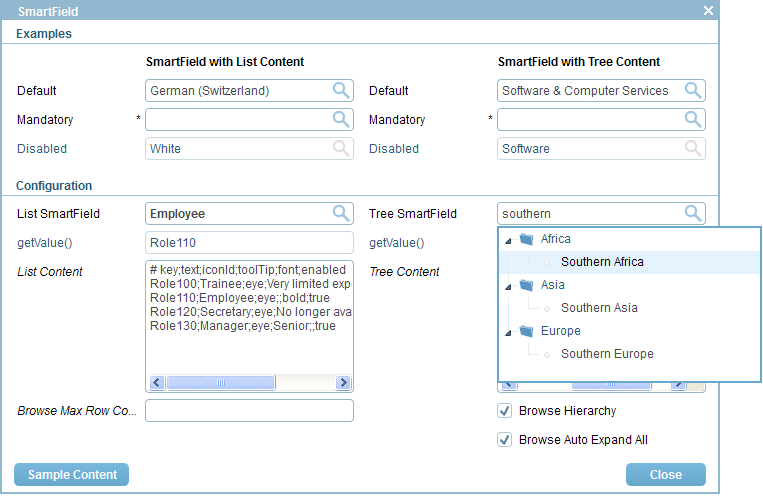
\includegraphics[width=14cm]{smartfield.png}
\caption{Smart field examples. 
Smart fields support ''search-as-you-type�� and are used to select a value from of a list of elements or a tree.}
\figlabel{smartfield}
\end{figure}

Example use cases for smart fields are provided in class \java{SmartFieldForm} of the Scout widget application and a screenshot of this example form is shown in \figref{smartfield}. 
The left hand side of the demo form contains smart fields based on list content and on the right hand side smart fields backed with hierarchical content are shown. 
In the example section of the demo form, some smart fields are backed by code types and others by lookup calls. 
And in the configuration section the content shown in the smart fields can be entered manually at runtime. 
To obtain the content shown in \figref{smartfield}, use the \button{Sample Content}. 

\noindent Existing Documentation
\begin{itemize}
  \item presentation: \url{http://wiki.eclipse.org/images/c/c9/20111102_EclipseConEurope2011-EclipseScout-DiscoverThePotential.pdf}
  \item forum: \url{http://www.eclipse.org/forums/index.php/t/369542/}
\end{itemize}

\subsection{Menus}
Each smart field can have menus attached. The menus will be shown when the user clicks on the \emph{arrow} symbol next to the smart field. Figure \ref{fig:smartfield_menu} shows an example of a smart field along with a set of menus.
\begin{figure}[!htb]
\centering
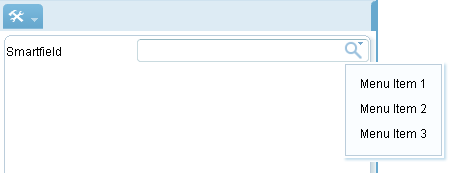
\includegraphics[width=0.8\textwidth]{smartfieldmenu.png}
\caption{Menus attached to a smart field.}
\label{fig:smartfield_menu}
\end{figure}

By default, the menus will only be shown if a value of the smart field has been selected. To show the menus even if the smart field is empty, one has to override the menu's \lstinline$getConfiguredEmptySpaceAction$ method:

% --------------------------------------------------------------------------- %
\section{Tree Field}
needs text

\begin{figure}
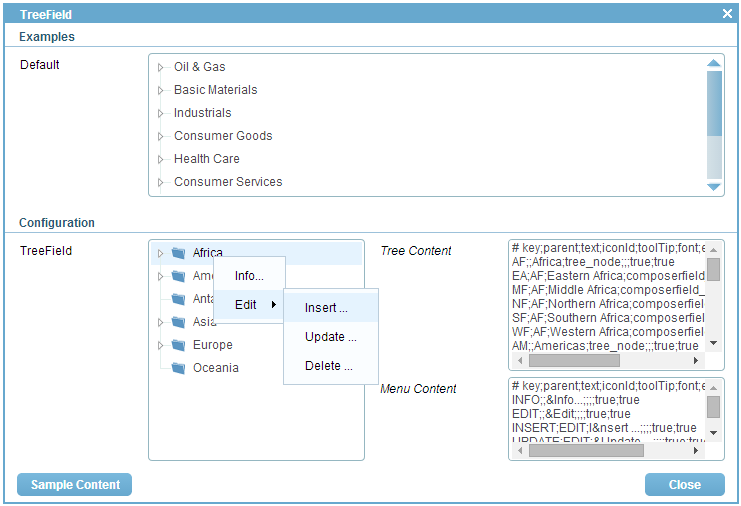
\includegraphics[width=15cm]{treefield.png}
\caption{Tree fields and example use cases.
More text.}
\figlabel{treefield}
\end{figure}

% --------------------------------------------------------------------------- %
\section{Table Field}
needs text

\begin{figure}
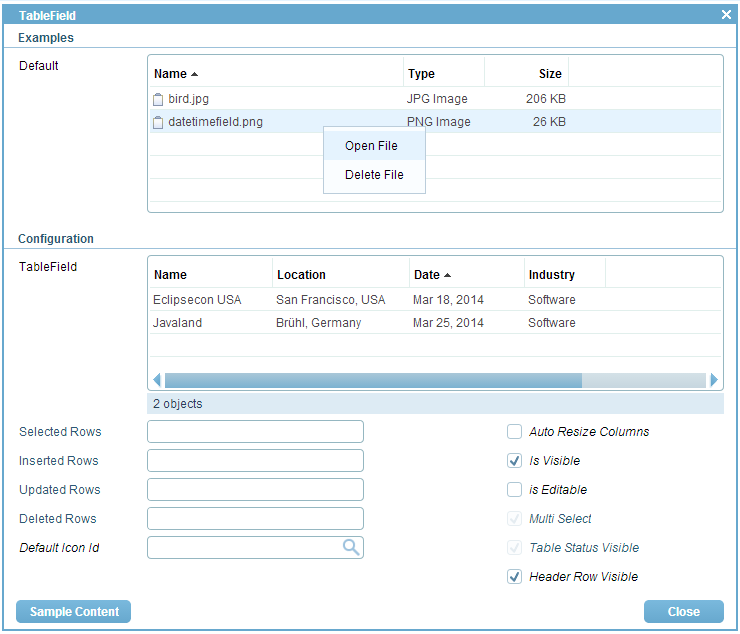
\includegraphics[width=15cm]{tablefield.png}
\caption{Table fields and example use cases.
More text.}
\figlabel{tablefield}
\end{figure}

\begin{figure}
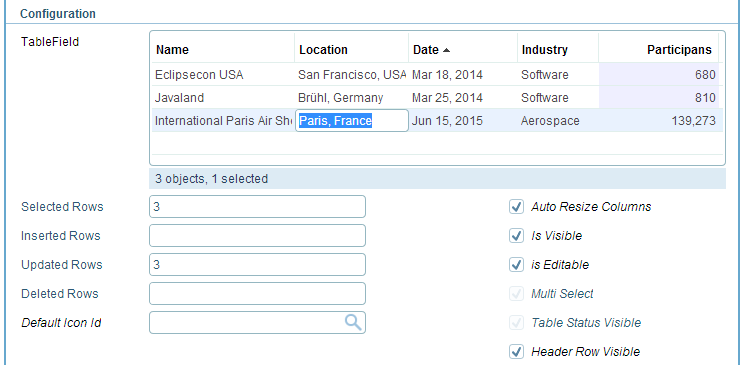
\includegraphics[width=15cm]{editabletablefield.png}
\caption{An editable table field.
More text.}
\figlabel{editabletablefield}
\end{figure}

\noindent Existing Documentation
\begin{itemize}
  \item wiki tutorial \url{http://wiki.eclipse.org/Scout/Tutorial/3.8/Minicrm/Table_Field}
  \item forum: \url{http://www.eclipse.org/forums/index.php/t/392053/}
  \item forum: load/save data \url{http://www.eclipse.org/forums/index.php/t/253311/}
\end{itemize}

% --------------------------------------------------------------------------- %
\section{Image Field}
needs text

\begin{figure}
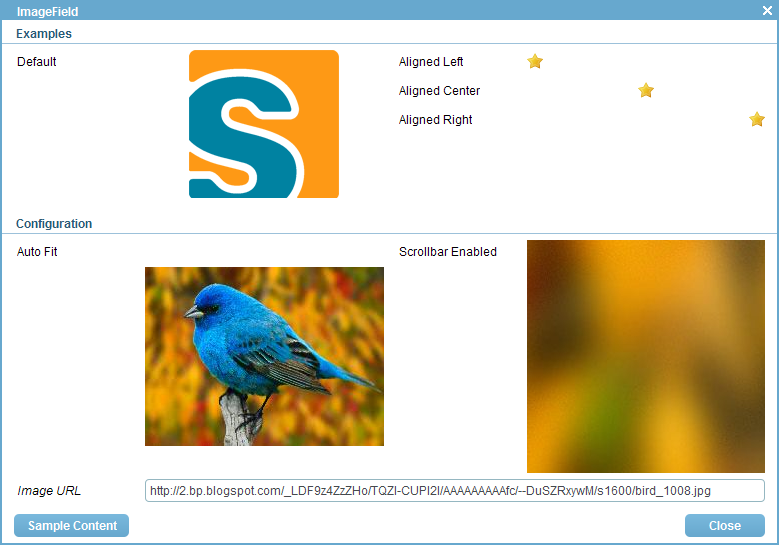
\includegraphics[width=14cm]{imagefield.png}
\caption{Image fields are used to display images and icons.
}
\figlabel{imagefield}
\end{figure}

\noindent Existing Documentation
\begin{itemize}
  \item forum: scrollbars \url{http://www.eclipse.org/forums/index.php/t/291205/}
\end{itemize}

% --------------------------------------------------------------------------- %
\section{SVG Field}
needs text

\begin{figure}
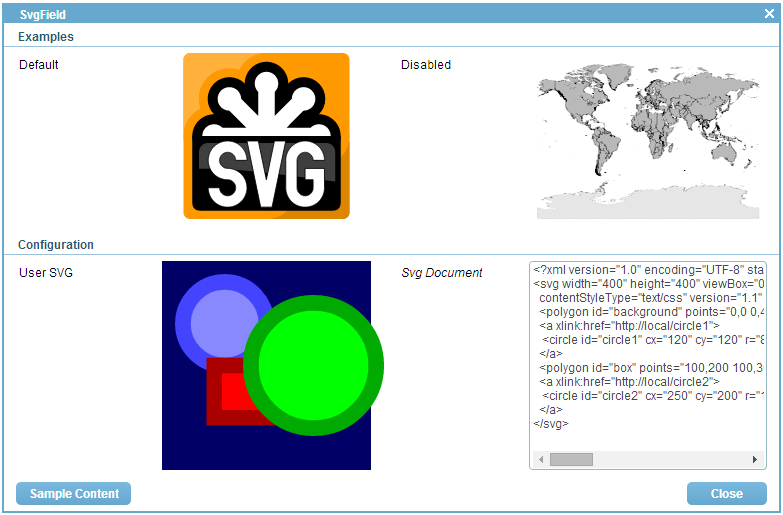
\includegraphics[width=15cm]{svgfield.png}
\caption{SVG fields and example use cases.
More text.}
\figlabel{svgfield}
\end{figure}

\noindent Existing Documentation
\begin{itemize}
  \item wiki tutorial \url{http://wiki.eclipse.org/Scout/Tutorial/3.8/SVG_Field}
\end{itemize}

% --------------------------------------------------------------------------- %
\section{HTML Field}
needs text

% --------------------------------------------------------------------------- %
\section{Browser Field}
needs text

\noindent Existing Documentation
\begin{itemize}
  \item forum: \url{http://www.eclipse.org/forums/index.php/t/414483/}, 
  \item forum: \url{http://www.eclipse.org/forums/index.php/t/369963/}, 
  \item forum: mozilla as default: \url{http://www.eclipse.org/forums/index.php/t/342433/}
\end{itemize}

% --------------------------------------------------------------------------- %
\section{Calendar Field}
needs text

\noindent Existing Documentation
\begin{itemize}
  \item forum: calendar field \url{http://www.eclipse.org/forums/index.php/t/370052/}
  \item forum: execloaditems \url{http://www.eclipse.org/forums/index.php/t/277447/}
  \item forum: filtering items \url{http://www.eclipse.org/forums/index.php/t/285644/}
  \item forum: usage example \url{http://www.eclipse.org/forums/index.php/t/265028/}
\end{itemize}

% =========================================================================== %
\chapter{Layout Widgets}
\chalabel{layoutwidgets}

% --------------------------------------------------------------------------- %
\section{Group Box}
needs text


\begin{figure}
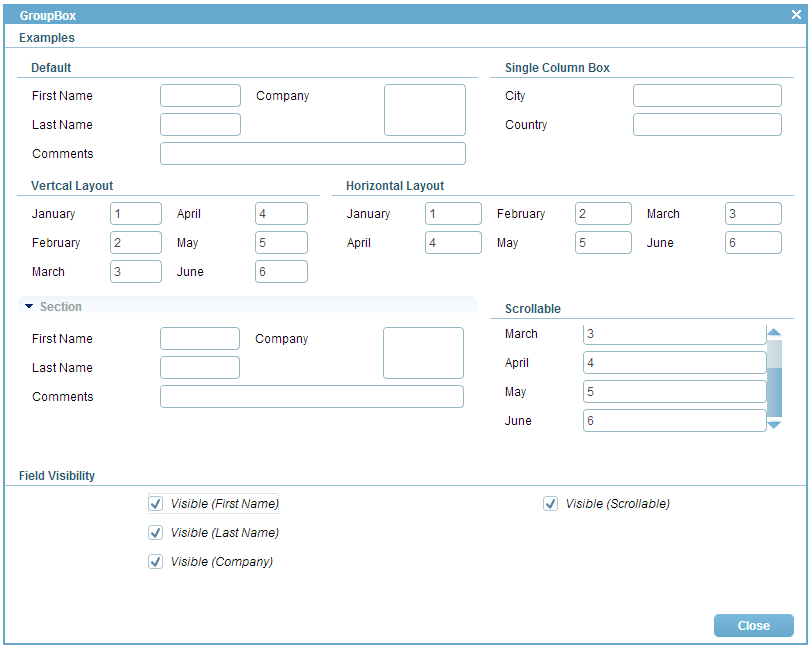
\includegraphics[width=15cm]{groupbox.png}
\caption{Group boxes and example use cases.
More text.}
\figlabel{groupbox}
\end{figure}

% --------------------------------------------------------------------------- %
\section{Tab Box}
needs text

\begin{figure}
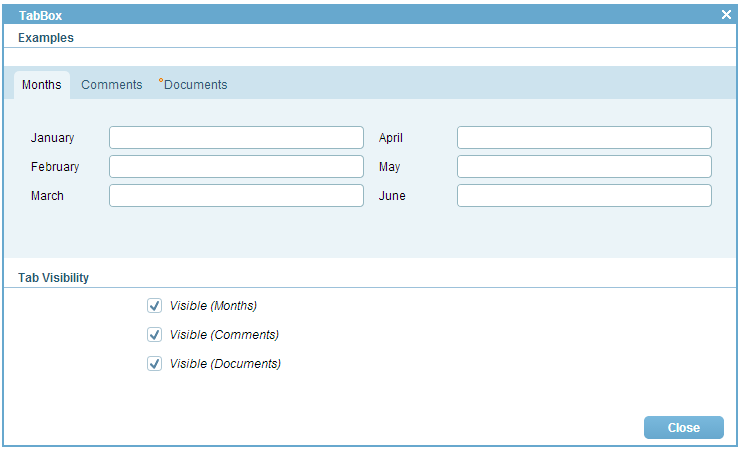
\includegraphics[width=15cm]{tabbox.png}
\caption{Tab boxes and example use cases.
More text.}
\figlabel{tabbox}
\end{figure}

% --------------------------------------------------------------------------- %
\section{Sequence Box}
needs text

\begin{figure}
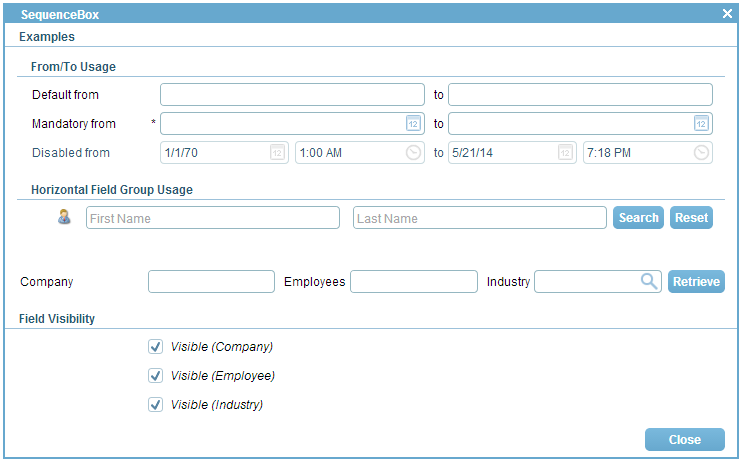
\includegraphics[width=15cm]{sequencebox.png}
\caption{Sequence boxes and example use cases.
More text.}
\figlabel{sequencebox}
\end{figure}

\noindent Existing Documentation
\begin{itemize}
  \item forum: \url{http://www.eclipse.org/forums/index.php/t/414629/}
\end{itemize}

* exec methods
* field validation

% --------------------------------------------------------------------------- %
\section{Split Box}
needs text

\begin{figure}
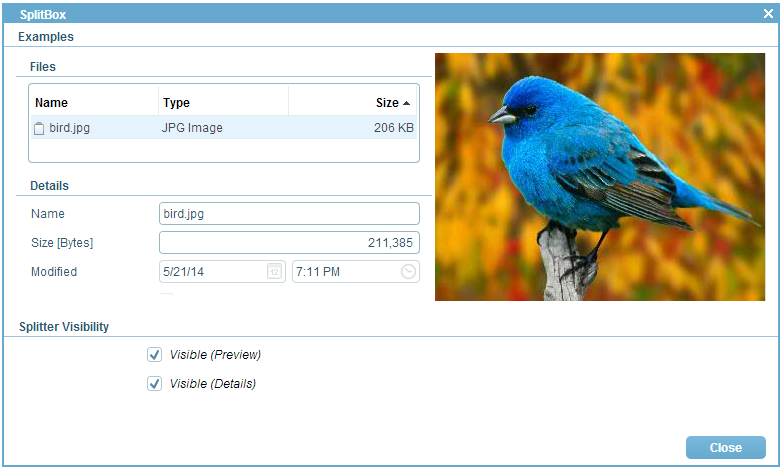
\includegraphics[width=15cm]{splitbox.png}
\caption{Split boxes and example use cases.
More text.}
\figlabel{splitbox}
\end{figure}


% --------------------------------------------------------------------------- %
\section{Page Field}
needs text

\noindent Existing Documentation
\begin{itemize}
  \item forum: \url{http://www.eclipse.org/forums/index.php/t/395360/}
\end{itemize}

% --------------------------------------------------------------------------- %
\section{File Chooser Field}
needs text

\noindent Existing Documentation
\begin{itemize}
  \item forum: file chooser field \url{http://www.eclipse.org/forums/index.php/t/377581/}
  \item forum: open with default file name: \url{http://www.eclipse.org/forums/index.php/t/351352/}
  \item how-to wiki: rap file chooser \url {http://wiki.eclipse.org/Scout/HowTo/3.8/Add_FileChooser_support_for_RAP_UI}
\end{itemize}

% --------------------------------------------------------------------------- %
\section{Master Slave Fields}
needs text

\noindent Existing Documentation
\begin{itemize}
  \item forum: \url{http://www.eclipse.org/forums/index.php/t/366931/}
\end{itemize}

% =========================================================================== %
\chapter{Custom Fields}
\chalabel{custom_fields}

As we have seen in the previous chapter, Scout already comes with a large amount of ready to use form fields. 
However, real life projects often need to meet special business requirements that can not be covered by the existing Scout form fields. 
For such situations the flexibility of the Scout framework allows the project to extend the exiting set of form fields with custom form fields. 

Custom form fields concists of a couple of components. Modeling and UI and registration and extension point?

\noindent Existing Documentation
\begin{itemize}
  \item how-to wiki: \url{http://wiki.eclipse.org/Scout/HowTo/3.8/Add_a_custom_GUI_component}
  \item forum: wrap existing javaview.de swing component \url{http://www.eclipse.org/forums/index.php/t/262755/}
\end{itemize}

  * concept
  * showcase: drawing application

% =========================================================================== %
\chapter{Template Fields}
needs text

\noindent Existing Documentation
\begin{itemize}
  \item concept wiki: \url{http://wiki.eclipse.org/Scout/Concepts/Template}
  \item forum: form data for template fields \url{http://www.eclipse.org/forums/index.php/t/261235/}
  \item forum: form ''modularisation'' \url{http://www.eclipse.org/forums/index.php/t/245857/}
\end{itemize}



% =========================================================================== %
\chapter{Layouting}
needs text

\noindent Existing Documentation
\begin{itemize}
  \item concept wiki \url{http://wiki.eclipse.org/Scout/Concepts/Client_Plug-In#Layouting}
\end{itemize}

% --------------------------------------------------------------------------- %
\section{The Desktop}
needs text

% --------------------------------------------------------------------------- %
\section{Form Layout}
needs text


% =========================================================================== %
\chapter{Bookmarks}
needs text

% =========================================================================== %
\chapter{Client Notification}
needs text

\noindent Existing Documentation
\begin{itemize}
  \item presentation: \url{http://wiki.eclipse.org/images/e/ea/20121022_BahBah_Slides.pdf}
  \item concept wiki: \url{http://wiki.eclipse.org/Scout/Concepts/Client_Notification}
  \item forum: \url{http://www.eclipse.org/forums/index.php/t/241053/}
\end{itemize}
      
% =========================================================================== %
\chapter{File Upload and Download}
needs text

\noindent Existing Documentation
\begin{itemize}
  \item how-to wiki: \url{http://wiki.eclipse.org/Scout/HowTo/3.8/Transfer_a_file_from_the_client_to_the_server}
  \item how-to wiki: \url{http://wiki.eclipse.org/Scout/HowTo/3.8/Use_RemoteFileService}
  \item forum with error message box exampl \url{http://www.eclipse.org/forums/index.php/t/441101/}
  \item forum: \url{http://www.eclipse.org/forums/index.php/t/368166/}
  \item forum: \url{http://www.eclipse.org/forums/index.php/t/366585/}
  \item forum: remotefileservice \url{http://www.eclipse.org/forums/index.php/t/266862/}
  \item forum: file download \url{http://www.eclipse.org/forums/index.php/t/263896/}
  \item forum: load \& display file \url{http://www.eclipse.org/forums/index.php/t/440934/}
\end{itemize}

% =========================================================================== %
\chapter{Application Branding}
needs text

\noindent Existing Documentation
\begin{itemize}
  \item forum: \url{http://www.eclipse.org/forums/index.php/t/373921/}
  \item forum: Splash \url{http://www.eclipse.org/forums/index.php/t/263003/}, 
  \item forum: Splash \url{http://www.eclipse.org/forums/index.php/t/164495/}
  \item forum: Login Box \url{http://www.eclipse.org/forums/index.php/t/417248/}
  \item forum: App Icon \url{http://www.eclipse.org/forums/index.php/t/263221/}
  \item forum: App Name \url{http://www.eclipse.org/forums/index.php/t/262121/}
  \item forum: Desktop \url{http://www.eclipse.org/forums/index.php/t/373921/}
  \item forum: Scout info form \url{http://www.eclipse.org/forums/index.php/t/236630/}
\end{itemize}

* Icons
* Fonts / Colors
* Look and Feel (Swing)

% --------------------------------------------------------------------------- %
\section{Rayo Look and Feel}
needs text

\noindent Existing Documentation
\begin{itemize}
  \item forum \url{http://www.eclipse.org/forums/index.php/t/369809/}
  \item wiki tutorial \url{http://wiki.eclipse.org/Scout/Tutorial/3.8/Rayo_Look_and_Feel}
\end{itemize}

% --------------------------------------------------------------------------- %
\section{Branding the Swing Client}
needs text

\noindent Existing Documentation
\begin{itemize}
  \item how-to wiki: for logo \url{http://wiki.eclipse.org/Scout/HowTo/3.8/Branding_the_Swing_Client}
  \item how-to wiki: app logo \url{http://wiki.eclipse.org/Scout/HowTo/3.8/Exchange_Default_Images}
\end{itemize}

% --------------------------------------------------------------------------- %
\section{Branding the SWT Client}
needs text

\noindent Existing Documentation
\begin{itemize}
  \item how-to wiki: for logo \url{http://wiki.eclipse.org/Scout/HowTo/3.8/Branding_the_Swing_Client}
  \item how-to wiki: app logo \url{http://wiki.eclipse.org/Scout/HowTo/3.8/Exchange_Default_Images}
\end{itemize}

% --------------------------------------------------------------------------- %
\section{Branding the Webclient}
needs text

\noindent Existing Documentation
\begin{itemize}
  \item forum \url{http://www.eclipse.org/forums/index.php/t/367983/}
\end{itemize}

% =========================================================================== %
\chapter{Advanced Topics}
needs text  

% --------------------------------------------------------------------------- %
\section{Modifying the UI at Runtime}
needs text

\noindent Existing Documentation
\begin{itemize}
  \item forum: inject fields in form \url{http://www.eclipse.org/forums/index.php/t/367124/}
\end{itemize}

% --------------------------------------------------------------------------- %
\section{Focus Handling}
needs text

\noindent Existing Documentation
\begin{itemize}
  \item forum: \url{http://www.eclipse.org/forums/index.php/t/369585/}
\end{itemize}

% --------------------------------------------------------------------------- %
\section{Keyboard Control}
needs text

\noindent Existing Documentation
\begin{itemize}
  \item forum: \url{http://www.eclipse.org/forums/index.php/t/351417/}
\end{itemize}

% --------------------------------------------------------------------------- %
\section{Master Detail Pages}
needs text

\noindent Existing Documentation
\begin{itemize}
  \item \url{http://www.eclipse.org/forums/index.php/t/405999/}
\end{itemize}

% --------------------------------------------------------------------------- %
\section{Client Only Applications}
needs text

\noindent Existing Documentation
\begin{itemize}
  \item how-to wiki: \url{http://wiki.eclipse.org/Scout/HowTo/3.8/Create_a_Standalone_Client_with_DB_Access}
  \item forum: client only \url{http://www.eclipse.org/forums/index.php/t/210183/}
  \item forum: offline capable client \url{http://www.eclipse.org/forums/index.php/t/210183/}
\end{itemize}


% --------------------------------------------------------------------------- %
\section{Headless Client}
needs text

\noindent Existing Documentation
\begin{itemize}
  \item headless client forum \url{http://www.eclipse.org/forums/index.php/t/262563/}
\end{itemize}

% --------------------------------------------------------------------------- %
\section{Client Startup}
needs text

\noindent Existing Documentation
\begin{itemize}
  \item reading command line parameters forum \url{http://www.eclipse.org/forums/index.php/t/281816/}
  \item do something right after login forum \url{http://www.eclipse.org/forums/index.php/t/261999/}
\end{itemize}

\subsection{Config.ini File}
needs text

\noindent Existing Documentation
\begin{itemize}
  \item config ini file forum \url{http://www.eclipse.org/forums/index.php/t/365140/}
  \item os independent *product/confg.ini forum \url{http://www.eclipse.org/forums/index.php/t/261674/}
\end{itemize}

% --------------------------------------------------------------------------- %
\section{Client Shutdown}
needs text

% --------------------------------------------------------------------------- %
\section{Threading and Jobs}
needs text

\noindent Existing Documentation
\begin{itemize}
  \item threading and jobs concept wiki \url{http://wiki.eclipse.org/Scout/Concepts/Client_Plug-In#Threading_and_Jobs}
\end{itemize}


% --------------------------------------------------------------------------- %
\section{Caching}
needs text

% --------------------------------------------------------------------------- %

\ifx\wholebook\relax\else
   \begin{thebibliography}{99}
  \addcontentsline{toc}{chapter}{Bibliography}
  
  % add/insert books in alphabetical order of 1st author
  
  \bibitem{batessierra05}
    \textit{Bert Bates, Kathy Sierra},
	\textbf{Head First Java} 2nd edition, 
	O'Reilly Media, 2005.

  \bibitem{bloch08} 
    \textit{Joshua Bloch},
    \textbf{Effective Java} 2nd edition, 
	Addison-Wesley, 2008.
	
  \bibitem{eckel06}
    \textit{Bruce Eckel},
	\textbf{Thinking in Java} 4th edition, 
	Prentice Hall International, 2006.

\end{thebibliography}

   \end{document}
\fi

% =========================================================================== %
